\documentclass[a4paper,11pt]{article}

\usepackage[utf8]{inputenc}
\usepackage{caption}
\usepackage[spanish]{babel}
\usepackage{fontenc}
\usepackage{graphicx}
\graphicspath{{figures/}}
\usepackage{verbatim}
\usepackage{listings}
\usepackage{fancyvrb,newverbs}
\usepackage{xcolor}
\usepackage{float}
\usepackage{amssymb,amsmath}
\usepackage[dvips]{hyperref}

\definecolor{bg}{gray}{0.93}
\newenvironment{cverbatim}
 {\SaveVerbatim{cverb}}
 {\endSaveVerbatim
  \flushleft\fboxrule=0pt\fboxsep=.5em
  \colorbox{bg}{\BUseVerbatim{cverb}}%
  \endflushleft
}

\newverbcommand{\cverb}
  {\setbox\verbbox\hbox\bgroup}
  {\egroup\colorbox{bg}{\box\verbbox}}
  
  % Title Page
\title{Manual de instalación y uso del plugin QGIS para preprocesar y ejectutar TSEB}
  
\date{\vspace{-5ex}}

\author{\vspace{-5ex}}

\begin{document}

\maketitle

\section{Instalación del complemento QGIS}\label{sec:configuracion}
Vamos a instalar el complemento de QGIS. Éste nos permitirá realizar cálculos y procesamiento de datos complejos, como es preparar los datos de entrada en los modelos de ET así como ejecutar el modelo de ET con el que trabajaremos. 

\subsection{Instalación de librerías externas}
Este complemento requiere de una serie de liberías externas a QGIS, que antes tenemos que instalar nosotros. El material de la práctica incluye un archivo de texto \cverb+requirements.txt+ y una subcarpeta \cverb+qgis-et-models-plugin+ que contiene el archivo comprimido \cverb+qgis-et-models.zip+.

Según tu sistema operativo sea Windows o Linux, sigue los pasos correspondientes.

\subsubsection{Windows}
\begin{enumerate}
 \item En la carpeta de Escritorio de QGIS o en los accesos directos de Inicio ejecuta \cverb+OSGeoW Shell+. Aparecerá una terminal MS-DOS.
 
 \item navega a la carpeta donde se encuentre el archivo \cverb+requirements.txt+. Para ello usa el comando \cverb+cd path\a\la\carpeta\+.
 
 \item Ejectua este comando\\\cverb+python -m pip install -r requirements.txt+
 
 Python empezará a instalar todas las librerías necesarias e indicadas por el archivo \cverb+requirements.txt+
\end{enumerate}

\subsubsection{Linux}
\begin{enumerate}
 \item Abre una Terminal, por ejemplo presinando \cverb|CTRL+ALT+T|.
 
 \item navega a la carpeta donde se encuentre el archivo \cverb+requirements.txt+. Para ello usa el comando \cverb+cd path/a/la/carpeta\+.
 
 \item Ejectua este comando\\\cverb+/usr/bin/python3 -m pip install -r requirements.txt+
 
 Python empezará a instalar todas las librerías necesarias e indicadas por el archivo \cverb+requirements.txt+
\end{enumerate}

\subsection{Instalación del complemento QGIS-ET-MODELS}
Cuando se hayan instalado estos requisitos previos, cierra la Terminal y abre QGIS.

\begin{enumerate}
 \item Pincha en \cverb+Complementos+\footnote{Plugins} $\rightarrow$ \cverb+Administrar e instalar complementos+\footnote{Manage and Install Plugins}.
 
 \item Activa la opción \cverb+Instalar a partir de ZIP+\footnote{Install from ZIP}.
 
 \begin{figure}[H]\centering
  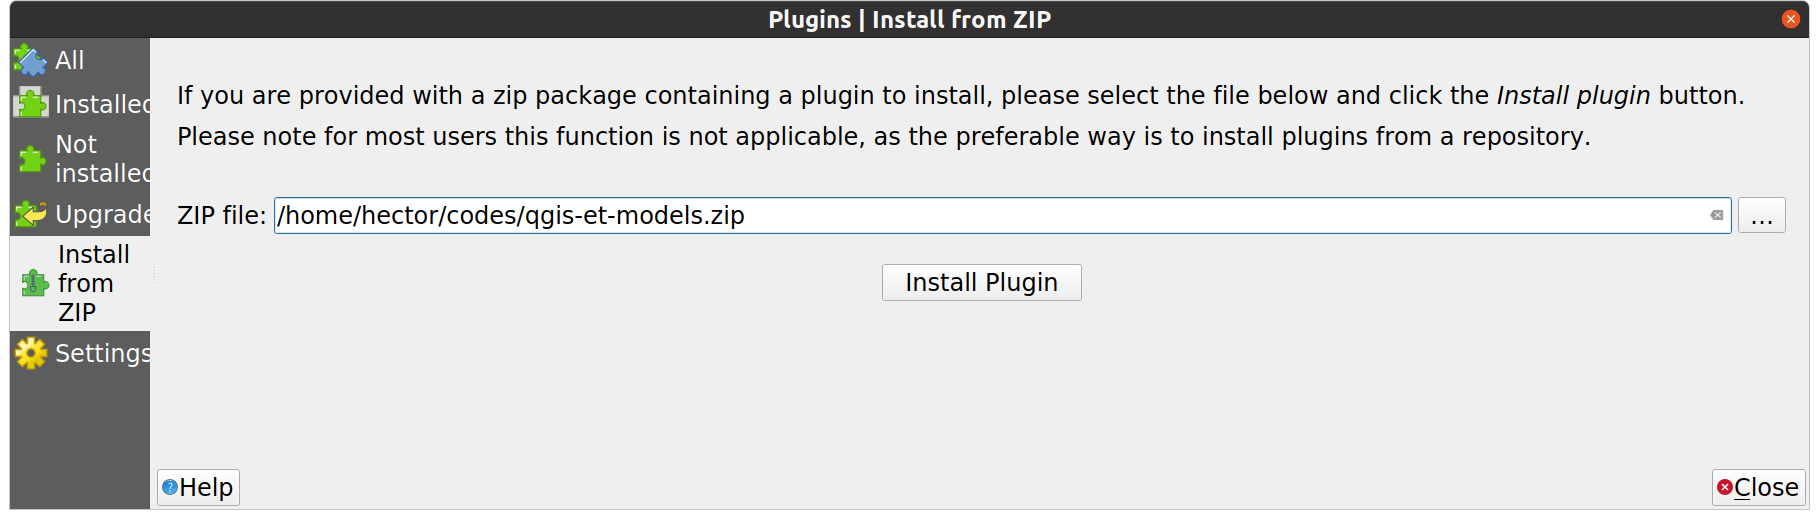
\includegraphics[width=\textwidth]{qgis_plugin_zip}
 \end{figure}

 
 \item navega hasta donde hayas guardado el archivo \cverb+qgis-et-models.zip+, selecciónalo y pincha en \cverb+Instalar complemento+\footnote{Install Plugin}
\end{enumerate}

Tardará un rato, pero al final deberías recibir un mensaje que el complemento ha sido instalado. Éste aparecerá en la Caja de herramientas de Procesos, bajo el nombre de \cverb+Evapotranspiration Processor+.
 \begin{figure}[H]\centering
  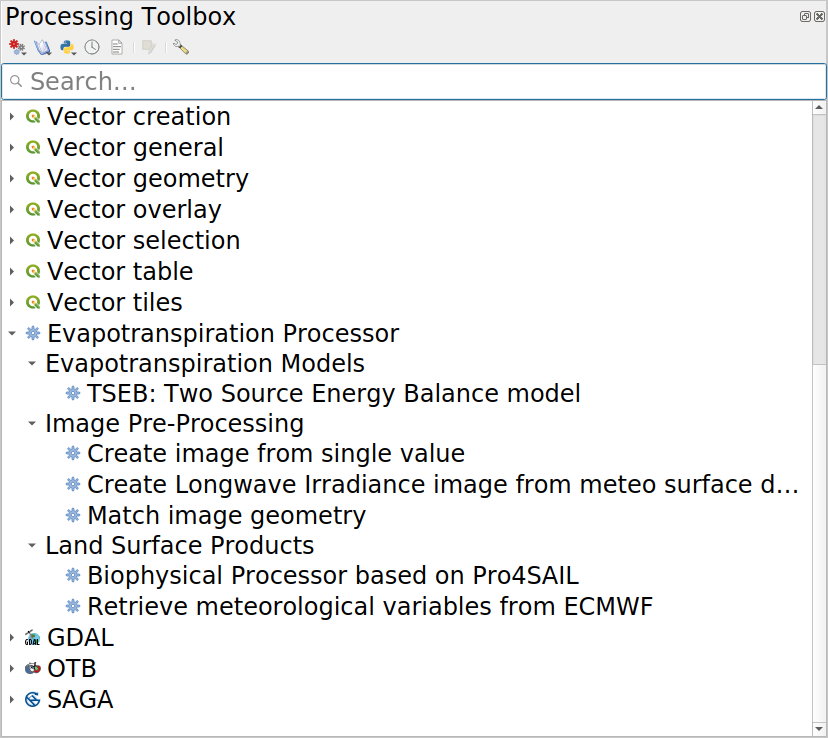
\includegraphics[width=\textwidth]{qgis_et_model_provider}
 \end{figure}


\section{Copernicus Climate Data Store y Atmosphere Data Store}\label{sec:ecmwf}
Los servicios Copernicus \href{https://cds.climate.copernicus.eu}{Climate Data Store}\footnote{\url{https://cds.climate.copernicus.eu}} y \href{https://ads.atmosphere.copernicus.eu}{Atmospheric Data Store}\footnote{\url{https://ads.atmosphere.copernicus.eu}} son dos aplicaciones web que ofrece la Unión Europea, a través de su programa Copernicus, para el acceso a los datos meteorológicos y climáticos generados por el Centro Europeo de predicción meteorológica a medio plazo (ECMWF). El acceso a los datos es gratuito pero es necesario registrarse previamente. Si no lo has hecho anteriormente regístrate \href{https://cds.climate.copernicus.eu/user/register?}{aquí}\footnote{\url{https://cds.climate.copernicus.eu/user/register?}} y \href{https://ads.atmosphere.copernicus.eu/user/register?}{aquí}\footnote{\url{https://ads.atmosphere.copernicus.eu/user/register?}}. 

Estos datos son una alternativa muy valiosa a las estaciones agrometerológicas, ya que para usar estas últimas en grandes superficies es necesario realizar tareas de interpolación espacial que pueden aportar mayores incertidumbres que las propias salidas de los modelos meteorológicos generados por el ECMWF u otros centros similares. 

Los reanálisis \href{https://cds.climate.copernicus.eu/cdsapp#!/dataset/reanalysis-era5-single-levels}{ERA-5} suponen uno de los datos meteorológicos geospaciales de mayor calidad. Son generados a través de modelos que han sido corregidos y re-calibrado a través de observaciones de estaciones meteorológicas a lo largo de todo el Globo, así como de información satelital, sondas meteorológicas y otras fuentes de datos adicionales. Si quieres saber más pincha \href{https://confluence.ecmwf.int/display/CKB/ERA5\%3A+data+documentation#ERA5:datadocumentation-Observations}{aquí}\footnote{\url{https://confluence.ecmwf.int/display/CKB/ERA5\%3A+data+documentation#ERA5:datadocumentation-Observations}}.

Estos productos representan datos meteorológicos horarios desde 1950 a $\approx$25km de resolución. Cubren todo el Globo tanto para superficies terrestres como marinas. Además tienen una latencia de tan sólo 5 días de retraso, lo que permiten su uso en tiempo casi-real. Además, pasados los tres meses los datos son revisados y reanalizados, mejorando su calidad con respecto a los datos en tiempo casi-real.

Sin embargo utilizar directamente estos datos no es del todo fácil. Los archivos que proporcionan vienen en formato NetCDF, que pueden llegar a tener un gran nivel de complejidad, ya que incluyen no sólo información geoespacial sino también temporal. Si abrieses los archivos directamente con QGIS como raster, verás que te pide varias opciones, como el tipo de variable (Dataset) que quieras abrir. Además te mostrará el producto como bandas, cada banda representa un periodo de tiempo (p.ej. una hora para ERA-5). 

Para trabajar mejor con éstos datos y corregirlos para obtener una mejor resolución espacial que la original, hemos desarrollado una herramienta en QGIS para automatizar todo el proceso de descarga y pre-procesamiento de los datos meteo, y así dejarlos listos para su introducción en los modelos que usaremos. Para ello sigue los siguientes pasos. Puedes saltar directamente al paso 6 si ya tienes configurados los archivos \cverb+.cdsapirc+ y \cverb+.adsapirc+.

\begin{enumerate}
  \item Ve a tu carpeta de usuario (en Linux esa carpeta es \cverb+/home/nombre_usuario+, y en Windows suele ser \cverb+C:\\Users\nombre_usuario+.
  
  \item Si no tienes la sesión abierta, inicia tu sesión en \url{https://cds.climate.copernicus.eu/user/login?} y luego introduce la siguiente dirección \url{https://cds.climate.copernicus.eu/api-how-to\#install-the-cds-api-key}
  
  \item Crea un archivo en blanco llamado \cverb+.cdsapirc+ (\emph{importante el punto al inicio}) y pega las dos lineas que te aparecen en el recuadro negro:
  \begin{figure}[H]\centering
    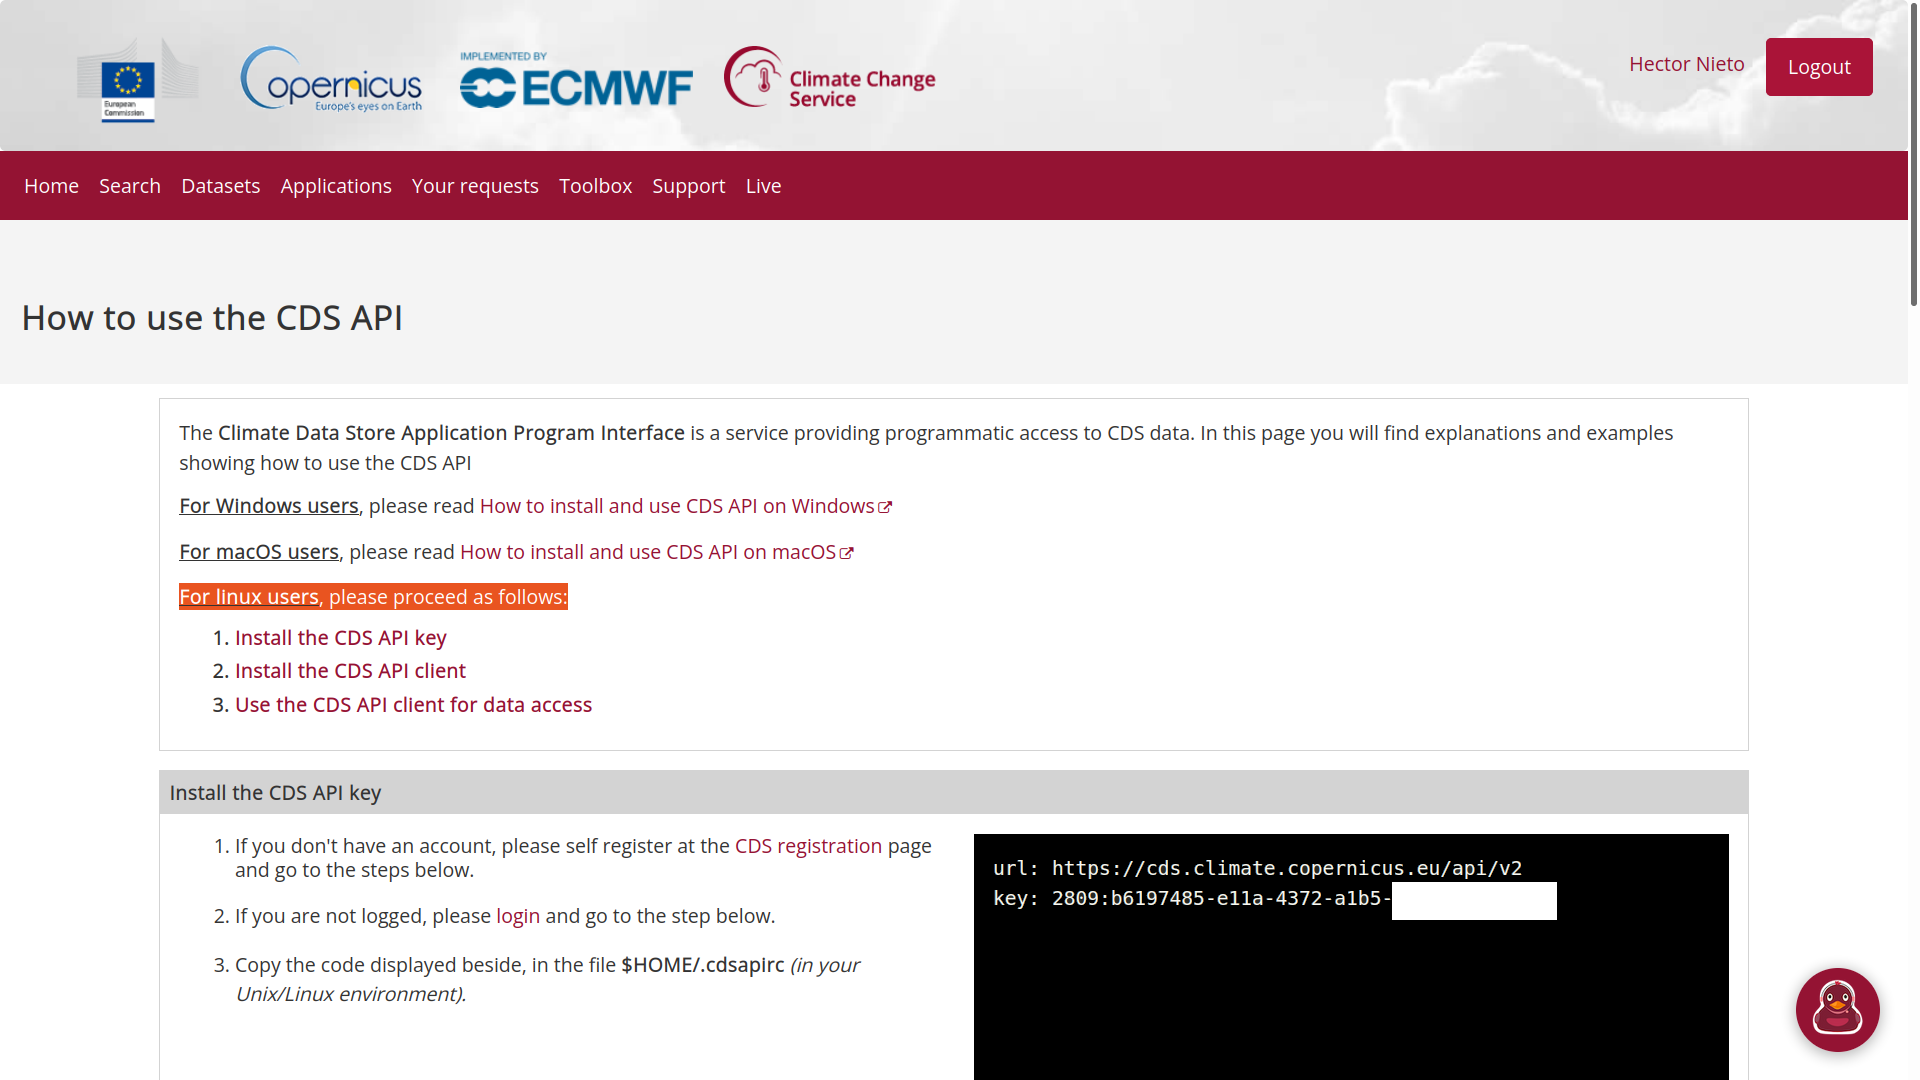
\includegraphics[width=\textwidth]{cds_key}
  \end{figure}
  
  Estas dos líneas tienen el siguiente formato
  \begin{cverbatim}
   url: https://cds.climate.copernicus.eu/api/v2
   key: UID:API-KEY
  \end{cverbatim}
  donde \cverb+UID+ y \cverb+API-KEY+ son tus identificadores de Copernicus Climate Data Store. También puedes obtenerlos viendo tu perfil de usuario.

  \item Si no tienes la sesión abierta, inicia ahora tu sesión en \url{https://ads.atmosphere.copernicus.eu/user/login?} y luego introduce la siguiente dirección \url{https://ads.atmosphere.copernicus.eu/api-how-to}
  
  \item Crea un archivo en blanco llamado \cverb+.adsapirc+ (\emph{importante el punto al inicio}) y pega las dos lineas que te aparecen en el recuadro negro al igual que hiciste anteriormente:
  
  Estas dos líneas tienen el siguiente formato
  \begin{cverbatim}
   url: https://ads.atmosphere.copernicus.eu/api/v2
   key: UID:API-KEY
  \end{cverbatim}
  donde \cverb+UID+ y \cverb+API-KEY+ son tus identificadores de Copernicus Atmospheric Data Store. También puedes obtenerlos viendo tu perfil de usuario.
  
  \item Vamos a ver si todo funciona. Abre QGIS, y si no lo tienes activado,
activa el plugin \cverb+Evapotranspiration Processor+

  \item En el panel de \cverb+Processing Toolbox+, ejecuta la herramienta \\\cverb+Evapotranspiration Processor+ \\$\rightarrow$ \cverb+Land Surface Products+ \\$\rightarrow$ \cverb+Retrieve meteorological variables from ECWMF+. Aparecerá un cuadro de diálogo como el siguiente:
  \begin{figure}[H]\centering
    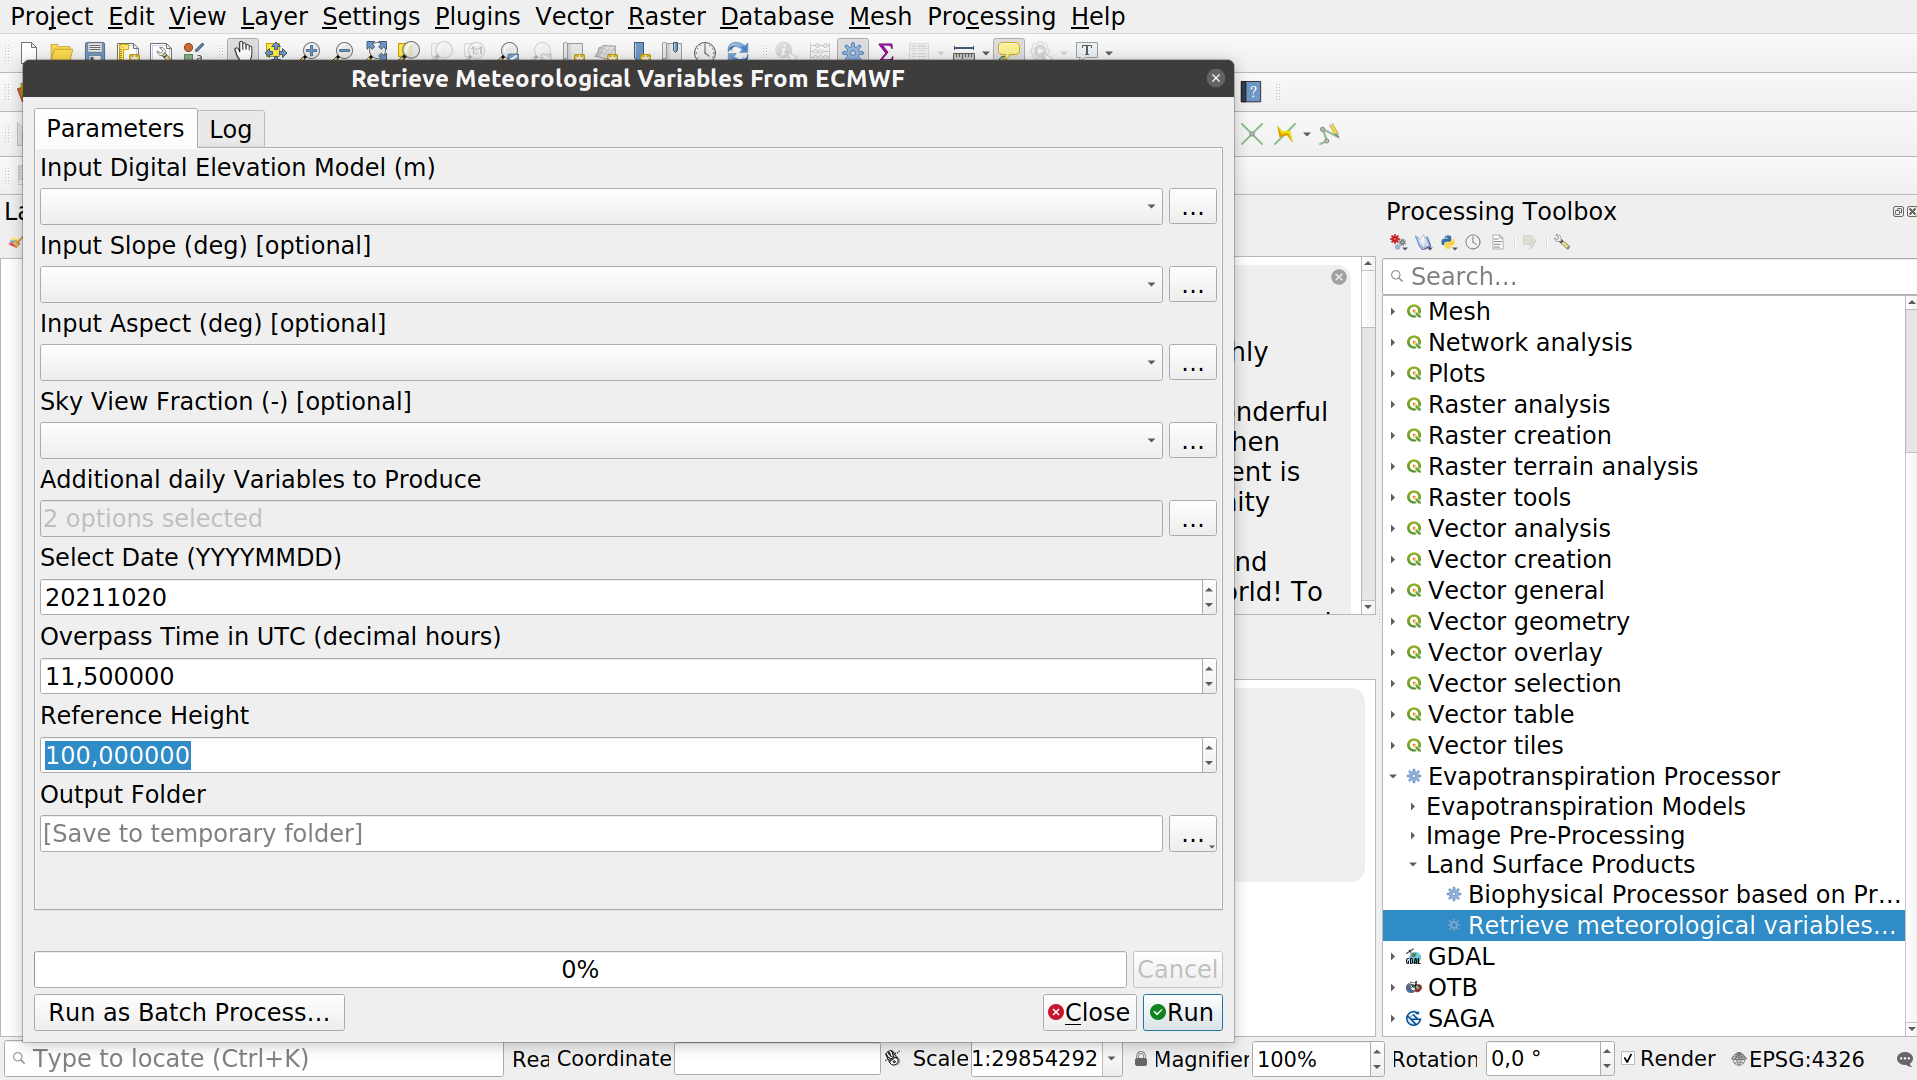
\includegraphics[width=\textwidth]{qgis_ecmwf}
  \end{figure}
  
  \item En \cverb+Input Digital Elevation Model (m)+ introduce el DTM que has procesado en la tarea anterior.
  
  \item En \cverb+Input Slope (deg) [optional]+ introduce el mapa de pendientes que has generado a partir del DTM anterior.
  
  \item En \cverb+Input Aspect (deg) [optional]+ introduce el mapa de exposiciones que has generado a partir del DTM anterior.
  
  \item En \cverb+Sky View Fraction (-) [optional]+ introduce el mapa de fracción de cielo visible que has generado a partir del DTM anterior.
  
  \item Deja \cverb+Additional daily Variables to Produce+ por defecto para calcular también la ET de referencia y la irradiancia solar diarias.
  
  \item En \cverb+Select Date (YYYYMMDD)+ introduce la fecha de adquisición, en formato AAAAMMDD, de una de las imágenes Landsat que te hayas descargado.
  
  \item En \cverb+Overpass Time (decimal hours)+ introduce la hora de adquisición, de una de las imágenes Landsat que te hayas descargado y que obtuviste gracias a los metadatos. La hora hay que introducirla en UTC y en hora decimal, por ejemplo 11.5 significa las 11:30 UTC.
  
  \item Deja \cverb+Reference Height (m)+ en el valor de 100m por defecto, ya que calcularemos las temperaturas y velocidades del viento a 100m sobre el nivel del suelo.
  
  \item En \cverb+Output Folder+ selecciona la carpeta donde quieres que se guarden las imágenes generadas. Te recomiendo al principio que crees una carpeta vacía y le des un nombre inequívoco (por ejemplo \cverb+meteo_AAAAMMDD+, con AAAAMMDD la fecha que quieres procesar).
  
  \item Pincha en \cverb+Run+. Recibirás varios mensajes del estado del proceso. Según el tamaño de tu DEM el proceso tardará más o menos tiempo mientras hace la consulta a los servidores de Copernicus, se descargan los datos y, finalmente, se corrijan:
  {\tiny \begin{cverbatim}
Parámetros de entrada:
{ 'ASPECT' : 'C:/Users/hectornieto/Downloads/data_test/data_test/aspect_utm.tif', 
'BLENDING_HEIGHT' : 100, 'DATE' : 20200605, 
'DEM' : 'C:/Users/hectornieto/Downloads/data_test/data_test/dem_utm.tif', 'OBJ_PARAM' : [0,1], 
'OUTPUT' : 'C:\\Users\\hectornieto\\Downloads\\data_test\\meteo_20200705', 
'SLOPE' : 'C:/Users/hectornieto/Downloads/data_test/data_test/slope_utm.tif', 
'SVF' : 'C:/Users/hectornieto/Downloads/data_test/data_test/svf_utm.tif', 'TIME' : 11.1 }

Downloading "100m_u_component_of_wind, 100m_v_component_of_wind, 
10m_u_component_of_wind, 10m_v_component_of_wind, 
2m_dewpoint_temperature, 2m_temperature, surface_pressure, 
surface_solar_radiation_downward_clear_sky, 
surface_solar_radiation_downwards, surface_thermal_radiation_downwards, 
total_column_water_vapour, geopotential" 
from the Copernicus Climate Store

Querying products for extent 43.99366771599999/-6.727821594/41.52203873699999/-4.0137665049999995
..and dates 2020-06-04 00:00:00 to 2020-06-06 00:00:00
{'format': 'netcdf', 
'variable': ['100m_u_component_of_wind', '100m_v_component_of_wind', 
'10m_u_component_of_wind', '10m_v_component_of_wind', 
'2m_dewpoint_temperature', '2m_temperature', 'surface_pressure', 
'surface_solar_radiation_downward_clear_sky',
'surface_solar_radiation_downwards','surface_thermal_radiation_downwards',
'total_column_water_vapour', 'geopotential'], 
'date': '2020-06-04/2020-06-06', 
'area': '43.99366771599999/-6.727821594/41.52203873699999/-4.0137665049999995', 
'product_type': 'reanalysis', 
'time': ['00:00', '01:00', '02:00', '03:00', '04:00', '05:00', '06:00', '07:00',
'08:00', '09:00', '10:00', '11:00', '12:00', '13:00', '14:00', '15:00', '16:00', 
'17:00', '18:00', '19:00', '20:00', '21:00', '22:00', '23:00']}

Saving into C:/Users/hectornieto/Downloads/data_test/meteo_20200705/era5_variables.nc
Saved to file C:/Users/hectornieto/Downloads/data_test/meteo_20200705/era5_variables.nc
Downloading "total_aerosol_optical_depth_550nm" from the Copernicus Atmospheric Store
Saved to file C:/Users/hectornieto/Downloads/data_test/meteo_20200705/cams_variables.nc
Computing Solar Zenith Angle
Processing ECMWF data for UTC time 2020-06-05 11:06:00
This may take some time...
Saving TA to C:/Users/hectornieto/Downloads/data_test/meteo_20200705\meteo_20200705_TA.tif
Saving EA to C:/Users/hectornieto/Downloads/data_test/meteo_20200705\meteo_20200705_EA.tif
Saving U to C:/Users/hectornieto/Downloads/data_test/meteo_20200705\meteo_20200705_U.tif
Saving P to C:/Users/hectornieto/Downloads/data_test/meteo_20200705\meteo_20200705_P.tif
Saving AOT to C:/Users/hectornieto/Downloads/data_test/meteo_20200705\meteo_20200705_AOT.tif
Saving TCWV to C:/Users/hectornieto/Downloads/data_test/meteo_20200705\meteo_20200705_TCWV.tif
Saving SDN to C:/Users/hectornieto/Downloads/data_test/meteo_20200705\meteo_20200705_SDN.tif
Saving SDNday to C:/Users/hectornieto/Downloads/data_test/meteo_20200705\meteo_20200705_SDNDAY.tif
Saving ETref to C:/Users/hectornieto/Downloads/data_test/meteo_20200705\meteo_20200705_ETREF.tif
Ejecución completada en 633.77 segundos
Resultados:
{'meteo_20200705_AOT.tif': 'C:/Users/hectornieto/Downloads/data_test/meteo_20200705\\meteo_20200705_AOT.tif',
'meteo_20200705_EA.tif': 'C:/Users/hectornieto/Downloads/data_test/meteo_20200705\\meteo_20200705_EA.tif',
'meteo_20200705_ETREF.tif': 'C:/Users/hectornieto/Downloads/data_test/meteo_20200705\\meteo_20200705_ETREF.tif',
'meteo_20200705_P.tif': 'C:/Users/hectornieto/Downloads/data_test/meteo_20200705\\meteo_20200705_P.tif',
'meteo_20200705_SDN.tif': 'C:/Users/hectornieto/Downloads/data_test/meteo_20200705\\meteo_20200705_SDN.tif',
'meteo_20200705_SDNDAY.tif': 'C:/Users/hectornieto/Downloads/data_test/meteo_20200705\\meteo_20200705_SDNDAY.tif',
'meteo_20200705_TA.tif': 'C:/Users/hectornieto/Downloads/data_test/meteo_20200705\\meteo_20200705_TA.tif',
'meteo_20200705_TCWV.tif': 'C:/Users/hectornieto/Downloads/data_test/meteo_20200705\\meteo_20200705_TCWV.tif',
'meteo_20200705_U.tif': 'C:/Users/hectornieto/Downloads/data_test/meteo_20200705\\meteo_20200705_U.tif'}
Cargando las capas resultantes
Algoritmo 'Retrieve meteorological variables from ECMWF' finalizado
  \end{cverbatim}}
\end{enumerate}

El sistema generará una imagen por producto meteorológico dentro de la carpeta seleccionada y además usara el nombre de la carpeta como patrón para nombrar a las imágenes.

\section{Preparación de los inputs}
  Según el modelo de ET de teledetección vamos a necesitar generar un mayor o menor número de inputs. En general cuanto más detallado, y potencialmente preciso, sea el modelo mayor número de inputs y, además, estos tendrían que ser de mejor calidad.

  Como hemos viniendo visto en prácticas anteriores, la variable clave es la temperatura de superficie, ya que ésta nos modula el grado de estrés hídrico, y por tanto cómo se reparte la energía disponible $R_n - G$ entre el flujo de calor sensible y el latente, o ET.

  \subsection{Preparación de la Temperatura de Superficie}
    Lo primero que vamos a hacer es recortar nuestra imagen de temperatura de superficie a la extensión de nuestra área de interés. Además el mapa de temperaturas de Landsat tiene los valores escalados. Esto quiere decir que generalmente a las imágenes y productos, para que ocupen menos espacio en el disco duro, se les aplica una transformación lineal con el fin de guardar los datos en números enteros. 
    
      \begin{equation}
        LST\left(K\right) = ADD + DN*MULT 
      \end{equation}
    donde $DN$ es el valor digital de la imagen, $ADD$ y $MULT$ son los factores de escalado y $LST\left(K\right)$ son los datos de temperatura de superficie originales.
    
    Para ello, como ya tenemos nuestro DTM recortado y reproyectado según nuestra área, podremos hacer lo siguiente:
    \begin{enumerate}
     \item En QGIS abre tanto el DTM recortado y reproyectado como la imagen Landsat \cverb+*_ST_B10.TIF+.
     
     \item ejecuta la función \cverb+Cortar raster por extensión+\footnote{Clip Raster by Extent}.
     
     \item En \cverb+Capa de entrada+\footnote{Input layer} selecciona tu imagen Landsat.
     
     \item En \cverb+Extensión de corte+\footnote{Clipping extent} selecciona \cverb+Calcular a partir de capa+\footnote{Calculate from raster} y elige el DTM.
     
     \item No toques nada en \cverb+Recortado (extensión)+\footnote{Clipped (extent)}, de modo que en el recuadro blanco diga \cverb+Guardar en archivo temporal+\footnote{{[Save to temporary file]}}. Esto lo haremos porque no queremos guardar en el disco esta imagen porque a continuación vamos a transformar sus valores originales en valores de temperatura.
    \end{enumerate}
    
    Al terminar el algoritmo podemos cerrar esa ventana y veremos nuestra nueva imagen recortada en el visor. Esta imagen que está en memoria, por lo que es un archivo temporal, ya que no queremos guardarla para el futuro. Lo que haremos ahora con ella es convertir los valores de la imagen en valores de temperatura (en Kelvin). 
    
    \begin{enumerate}
      \item Abre de nuevo los metadatos del producto Landsat (fichero con prefijo \cverb+MTL+) y busca un par de líneas conteniendo los textos\\ \cverb+TEMPERATURE_MULT_BAND_ST_B10+ y \cverb+TEMPERATURE_ADD_BAND_ST_B10+. Anota sus valores, ya que estos son los factores de escalado.
      
      \item Ejecuta la función \cverb+Calculadora ráster+\footnote{Raster Calculator} y transforma los valores del ráster que acabamos de recortar según la ecuación anterior:
      
      \cverb|ADD + "Clipped (extent)@1" * MULT|\\
     
      \item En \cverb+Capa de salida+\footnote{Output Layer} selecciona el nombre de archivo de salida. Con el fin de tener los datos ordenados, sugiero que lo guardes en una sub-carpeta, por ejemplo llamada \cverb+inputs_YYYYMMDD+\footnote{YYYYMMDD sería la fecha de adquisición}.
      
      \item Pincha en \cverb+OK+ para realizar los cálculos.
    \end{enumerate}
    
    Se creará una nueva imagen ya con los datos de temperatura reales. Puedes comprobar si los cálculos se han realizado correctamente si los valores de las temperaturas se encuentran dentro de valores esperables, como los 273 (~0ºC) y 320 (50 ºC). También puedes abrir la imagen de temperatura del aire que se generó en la práctica anterior (sufijo \cverb+TA+) y comparar que las diferencias entre \cverb+LST+ y \cverb+TA+ sean realistas.
  
  \subsection{Recorte de las otras bandas de Landsat}
    Ya tenemos nuestro primer input preparado para el modelo, que es la Temperatura de Superficie. Ahora lo que queremos es que el resto de los inputs que generemos tengan exactamente la misma geometría, es decir la misma extensión y resolución, para así permitir al modelo realizar los cálculos pixel a pixel. Hay un gran número de inputs y bandas a solapar, por lo que este proceso puede ser muy tedioso. Por fortuna, en nuestro complemento \cverb+Evapotranspiration Processor+ hemos desarrollado una función que nos va a facilitar mucho esta tarea.
    
    Vamos a remuestrear las otras bandas de Landsat, así como la banda de calidad \cverb+QA_PIXEL+ que usaremos en la siguiente tarea.
    
    \begin{enumerate}
     \item Ejecuta la herramienta \cverb+Match image geometry+ de \cverb+Evapotranspiration Processor+ $\rightarrow$ \cverb+Image Pre-Processing+.
     
     \begin{figure}[H]\centering
      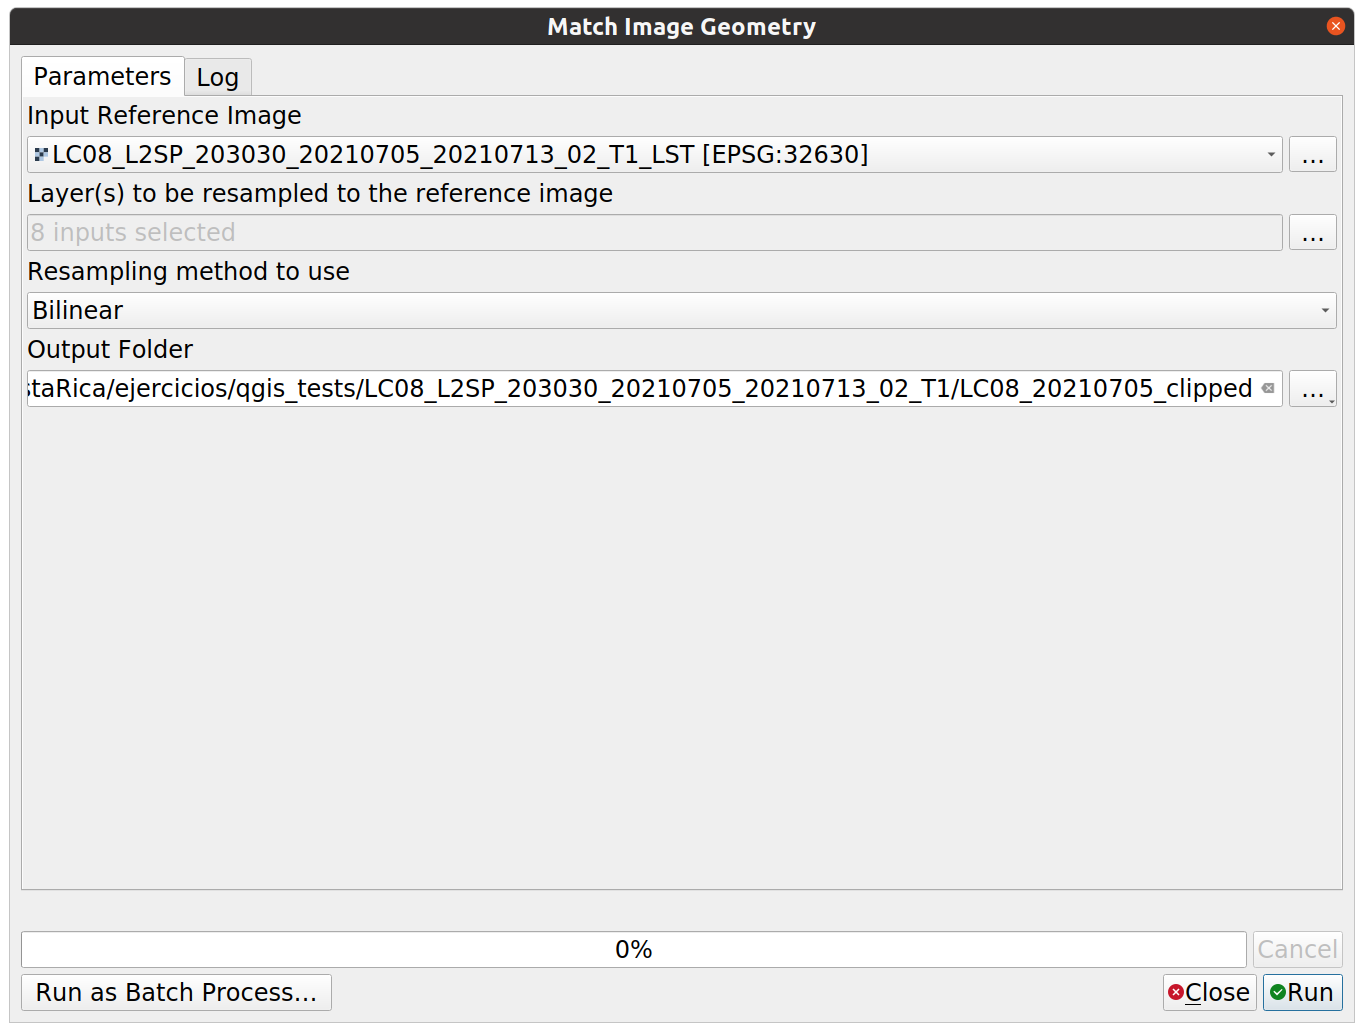
\includegraphics[width=\textwidth]{qgis_match_image_geometry}
     \end{figure}
     
     \item En \cverb+Input Reference Image+ selecciona nuestra imagen de temeperatura de superficie recortada, ya que es esta imagen sobre la que solaparemos el resto de los inputs.
     
     \item Pincha en el icono de los tres puntitos de\\ \cverb+Layer(s) to be resampled to the reference image+. Aparecerá un cuadro de diálogo en el que podrás seleccionar múltiples imágenes ya abiertas, múltiples archivos e incluso carpetas completas.
     
      \begin{figure}[H]\centering
      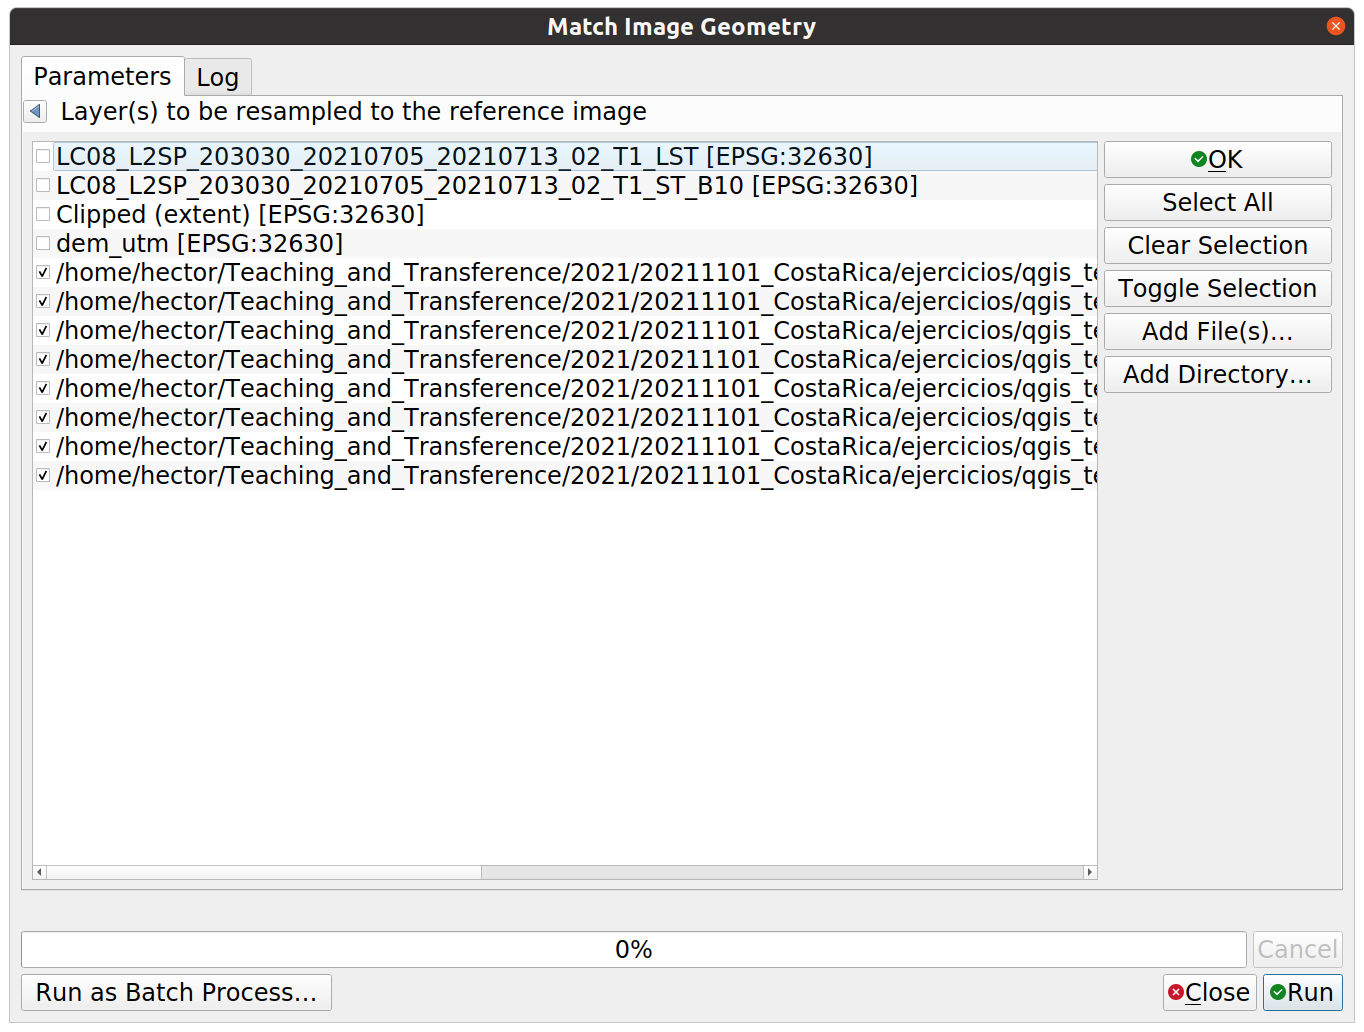
\includegraphics[width=\textwidth]{qgis_multiplefileselector}
     \end{figure}
      
      \item Pincha en \cverb+Add File(s)+ y navega a la carpeta donde tienes tu imagen Landsat original y selecciona los ficheros con los nombres \cverb+*_SR_B1.TIF+, \cverb+*_SR_B2.TIF+, \cverb+*_SR_B3.TIF+, \cverb+*_SR_B4.TIF+, \cverb+*_SR_B5.TIF+, \cverb+*_SR_B6.TIF+, \cverb+*_SR_B7.TIF+.
      
      \item Pincha en \cverb+OK+ cuando hayas terminado de seleccionar todos los archivos que quieras recortar.
      
      \item De nuevo en la ventana principal, selecciona \cverb+bilinear+ en \cverb+Resampling method to use+.
      
      \item Finalmente selecciona una carpeta de salida en \cverb+Output Folder+ donde se guardarán todas las imagens recortadas y ajustadas a la LST. Por ejemplo puedes usar la misma carpeta donde tienes guardada la imagen recortada de temperatura de superficie.
      
      \item Cuando tengas todo listo presiona \cverb+Run+ para ejecutar el proceso.
    \end{enumerate}
    
    Al terminar, el algoritmo habrá creado una serie de imágenes recortadas en la carpeta de salida, con el mismo nombre que la imagen original.
    
    Ahora vamos a repetir el proceso para \cverb+QA_PIXEL+. El motivo de no hacerlo junto con las bandas de reflectividad es que este ráster es un ráster cualitativo, y por tanto no podemos hacer un remuestreo bilinear, si no que es necesario remuestrear por el vecino más próximo.
    
    \begin{enumerate}
     \item Vuelve a ejecutar la herramienta \cverb+Match image geometry+.
     
     \item En \cverb+Input Reference Image+ selecciona nuestra imagen de temeperatura de superficie recortada.
     
     \item Pincha en el icono de los tres puntitos de\\ \cverb+Layer(s) to be resampled to the reference image+ y selecciona el fichero de la carpeta Landsat con el nombre \cverb+*_QA_PIXEL.TIF+.
      
      \item Pincha en \cverb+OK+.
      
      \item selecciona \cverb+Nearest Neighbour+ en \cverb+Resampling method to use+.
      
      \item Finalmente selecciona la carpeta de salida en \cverb+Output Folder+.
      
      \item Cuando tengas todo listo presiona \cverb+Run+ para ejecutar el proceso.
    \end{enumerate}
  
  \subsection{Máscara de Nubes}
    Es posible que tu imagen contenga nubes y sombras de nubes. En esos casos no queremos generar información para esos píxeles ya que son datos no válidos. Por fortuna los productos Landsat y Sentinel tienen su propia banda de calidad de los píxeles, en la que contiene información sobre presencia de nubes, sombras y/o cirros. Esta información está condificada de una manera que no es fácil interpretable directamente por un humano. En el caso de Landsat esta imagen es el fichero \cverb+QA_PIXEL+.
    
    En nuestro complemento también tenemos una herramienta para extraer la información de esa banda y generar una capa de presencia/ausencia de nubes y sombras (0 para presencia de nubes o sombras y 1 para píxels sin nubes ni sombras).
    
    \begin{enumerate}
     \item Ejecuta la herramienta\\ \cverb+Create Cloud Mask image from image quality data+
     \begin{figure}[H]\centering
      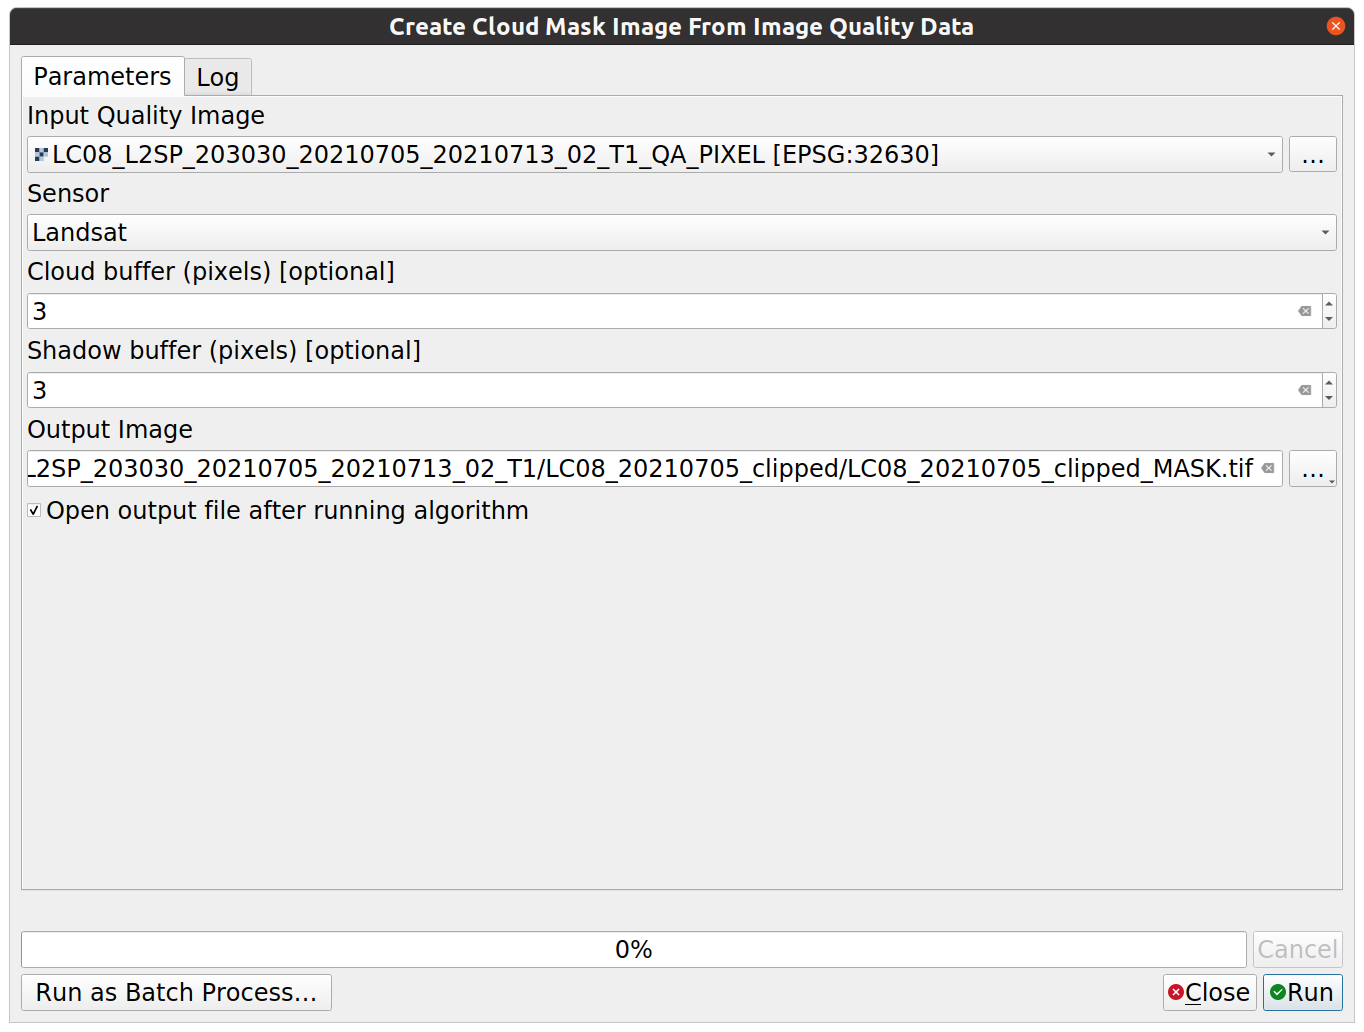
\includegraphics[width=\textwidth]{qgis_cloud_mask}
     \end{figure}
     
     \item En \cverb+Input Quality Image+ Selecciona la imagen \cverb+QA_PIXEL+ que acabamos de recortar acorde a nuestro mapa de temperatura.
     
     \item Selecciona \cverb+Landsat+ en \cverb+Sensor+ para decirle al algoritmo que esta banda de calidad se corresponde a una imagen Landsat.
     
     \item \cverb+Cloud buffer+ y \cverb+Shadow buffer+ son optativos. Le dice al algoritmo que elimine también los píxeles adyacentes a las nubes y las sombras, mediante un búffer. A veces estas regiones de transición entre la nube y las zonas soleadas no son muy claras de detectar si hay nube o no, por lo que es una forma de asegurarnos que la máscara elimina píxeles dudodos.
     
     \item En \cverb+Output Image+ selecciona el archivo de salida. Por ejemplo puedes usar un sufijo como \cverb+MASK+.
    \end{enumerate}
    
    El algoritmo transformará la imagen de calidad en una imagen con ceros y unos, donde sólo los píxeles de valor uno son píxeles con dato válido. Por ello en futuras tareas sólo se realizarán los cálculos en estos píxeles, ahorrándonos tiempo de procesamiento y evitando generar información errónea.
    
    \begin{figure}[H]\centering
     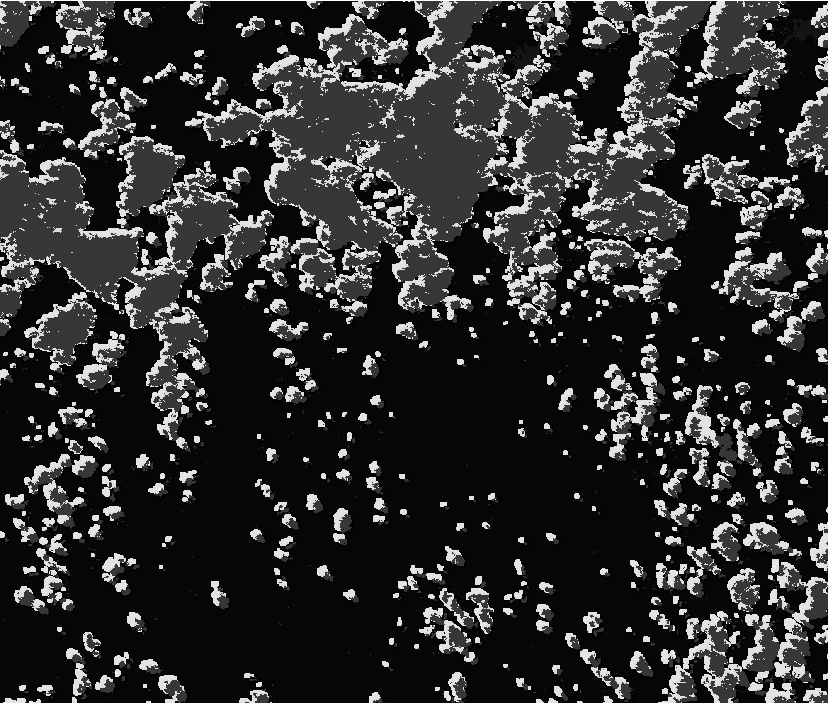
\includegraphics[width=0.45\textwidth]{qa_pixel}
     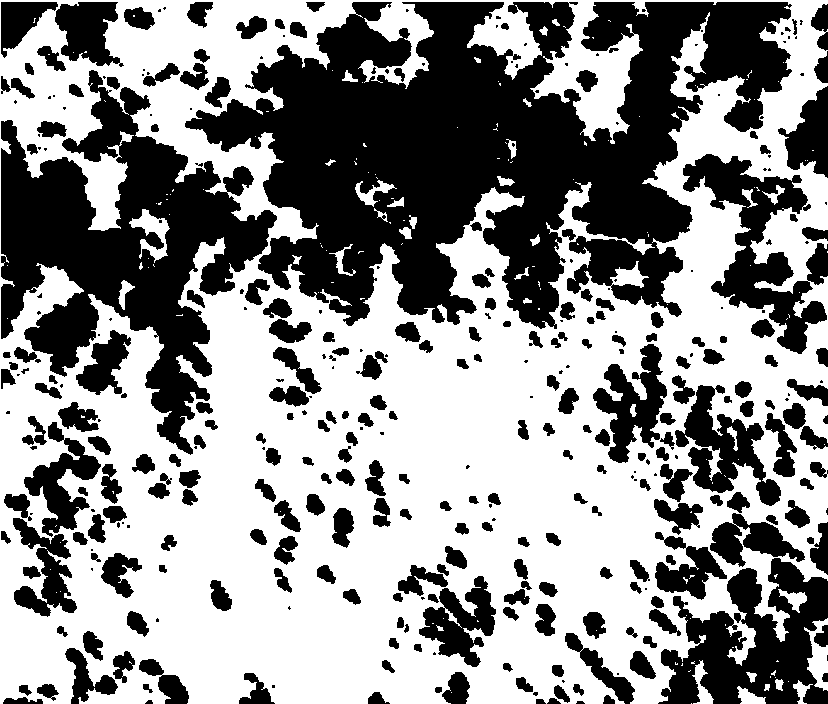
\includegraphics[width=0.45\textwidth]{mask_result}
    \end{figure}
    
  \subsection{Preparación de los parámetros biofísicos}
    Por otro lado también necesitamos derivar información fisiológica del cultivo mediante datos multiespectrales. Algunos modelos requieren apenas el cálculo del NDVI y el albedo, mientras que otros, como por ejemplo el modelo TSEB que usaremos, requieren de inputs más detallados:

    \begin{itemize}
      \item El Índice de Área Foliar ($LAI$). Nos determinará principalmente la fracción de radiación que es interceptada por el dosel vegetal, y por tanto la energía disponible que tiene la planta para transpirar y/o elevar su temperatura.
      
      \item El albedo de la superficie y/o los pigmentos de la hoja. Que nos determinará las propiedades espectrales de la planta y la superficie y por tanto, la radiación de onda corta que absorbe la planta.
      
      \item La fracción del LAI que es fotosintéticamente activa ($f_g$). Que nos determinará la fracción de radiación absorbida que potencialmente puede ser usada para la fotosíntesis y la transpiración.
      
      \item La altura de la vegetación ($h_c$). Que nos determinará la rugosidad de la superficie y por tanto el cálculo de las resistencias aerodinámicas.
      
      \item La fracción de suelo ocupada por el cultivo ($f_c$). Sólo para cultivos heterogéneos y/o en hileras, con una zona de suelo evidentemente expuesta. Se utilizaría para calcular el grado de agrupamiento de las copas.
    \end{itemize}

    En esta práctica, $LAI$, $f_g$ y pigmentos se van a derivar con los datos multiespectrales, mediante la inversión de un modelo de transferencia radiativa. Por otro lado $h_c$ y $f_c$ deben ser pre-establecido por el usuario en función el conocimiento de su cultivo y del manejo del mismo.

    \subsubsection{Derivación de parámetros biofísicos}
      Vamos a derivar $LAI$, $C_{a+b}$, $fAPAR$, $fIPAR$, así como el peso específico de la hoja $C_m$ y su contenido de agua `$C_w$. Según el sensor que vayamos a utilizar en el futuro (Landsat, Sentinel-2, ...) podremos estimar estos parámetros con mayor o menor incertidumbre, según la sensibilidad de sus bandas a variaciones de estas variables (siempre podrás acceder al cuaderno digital sobre el espectro en la plataforma \href{https://mybinder.org/v2/gh/hectornieto/Curso-WUE/HEAD}{MyBinder.org}).
      
      Para ello, en lugar de trabajar con índices de vegetación específicos, vamos a utilizar toda la información espectral que nos proporciona Landsat (o Sentinel en el futuro) con todas sus bandas. Antes de nada por lo tanto tendremos que juntar las imágenes individuales de cada una de las bandas en una única imagen con todas las bandas apiladas. Esta tarea ya la hicimos en el curso básico de QGIS (función \cverb+Combinar+\footnote{Merge}). Sin embargo ahora vamos a hacerlo un poco diferente. En lugar de usar la función \cverb+Combinar+ y crear un nuevo GeoTiff, vamos a generar un ráster virtual (VRT). Un archivo VRT en lugar de guardar una imagen apilada en GeoTIFF, permite generar una imagen apilada simplemente como referencia a los archivos individuales existentes en el disco duro. Esto nos permite ahorrar memoria, ya que ocupa mucho menos espacio.
      
      \begin{enumerate}
       \item Ejecuta la función \cverb+Construir ráster virtual+\footnote{Build Virtual Raster} de \cverb+Raster+ $\rightarrow$ \cverb+Miscelánea+.
       
       \item En \cverb+Capas de entrada+\footnote{Input layers} pincha en los tres puntitos. Aparecerá el típico cuadro de diálogo de QGIS para seleccionar múltiples archivos. Añade los archivos correspondientes a tu imagen Landsat recortada con los nombres de \cverb+SR_B1+ a \cverb+SR_B7+ (siete archivos correspondientes a las siete bandas espectrales). Asegúrate que están bien ordenados, en primer lugar la banda 1 y en último lugar la banda 7, ya que ese será el orden de apilamiento en la nueva imagen apilada. Si ves que las bandas no aparecen ordenadas, puedes pinchar y arrastrar el nombre de cada banda a la posición que desees.
       
       \begin{figure}[H]\centering
        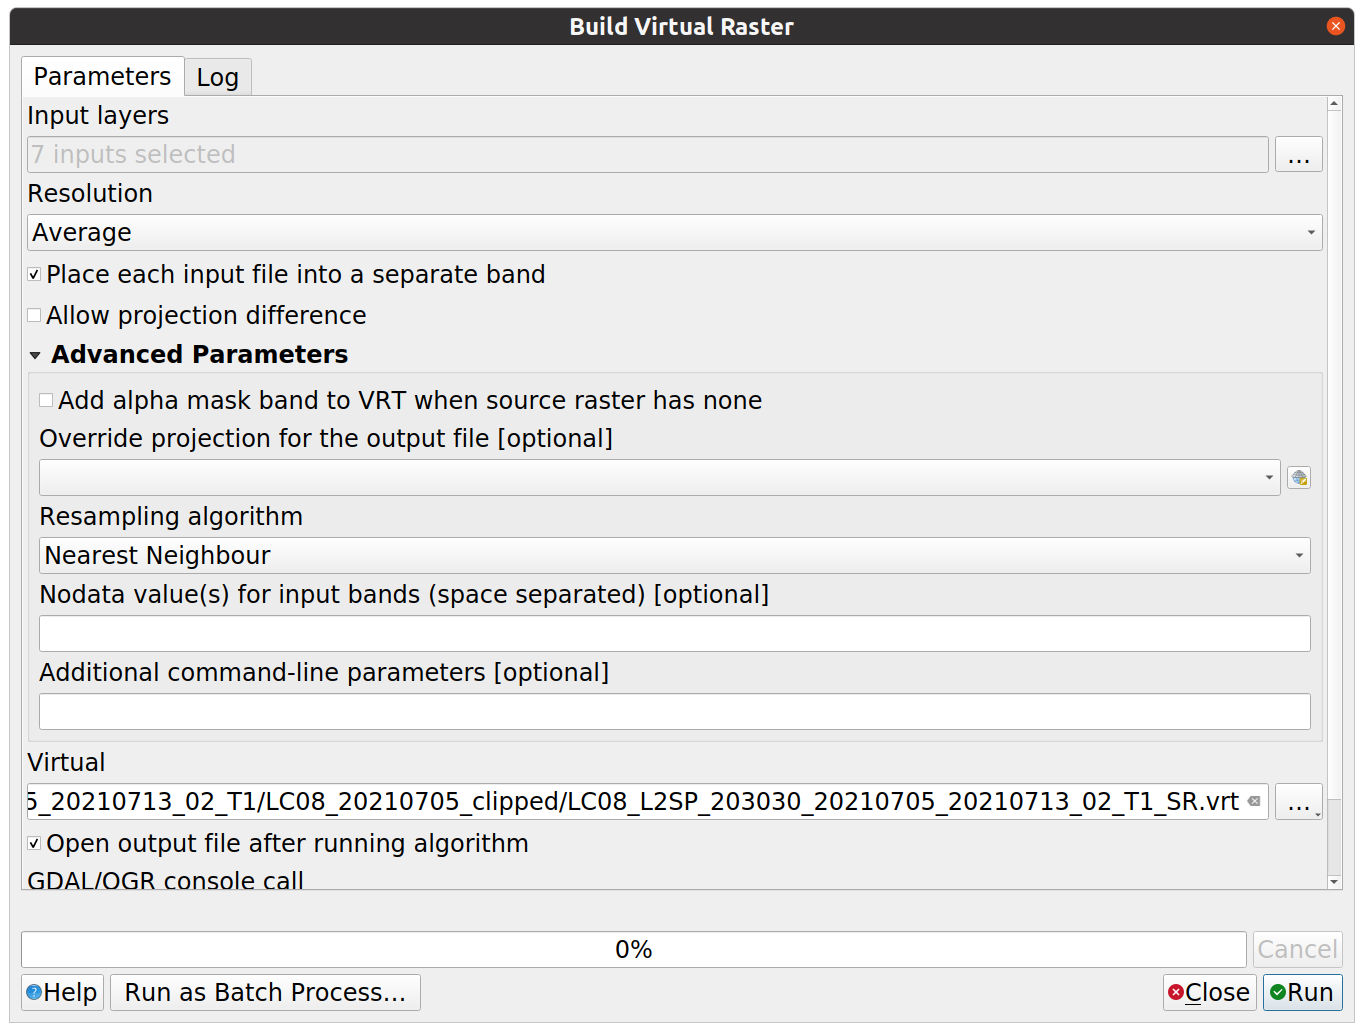
\includegraphics[width=\textwidth]{qgis_build_vrt}
       \end{figure}      
       
       \item Marca la opción \cverb+Coloque cada archivo de entrada en una banda separada+\footnote{Place each input file into a separate band}
       
       \item Deja el resto de opciones por defecto.
       
       \item En \cverb+Virtual+ vamos a seleccionar el archivo donde guardar el resultado, puedes guardar el archivo en la misma carpeta donde tienes tus imágenes recortadas. 
       
       \begin{figure}[H]\centering
        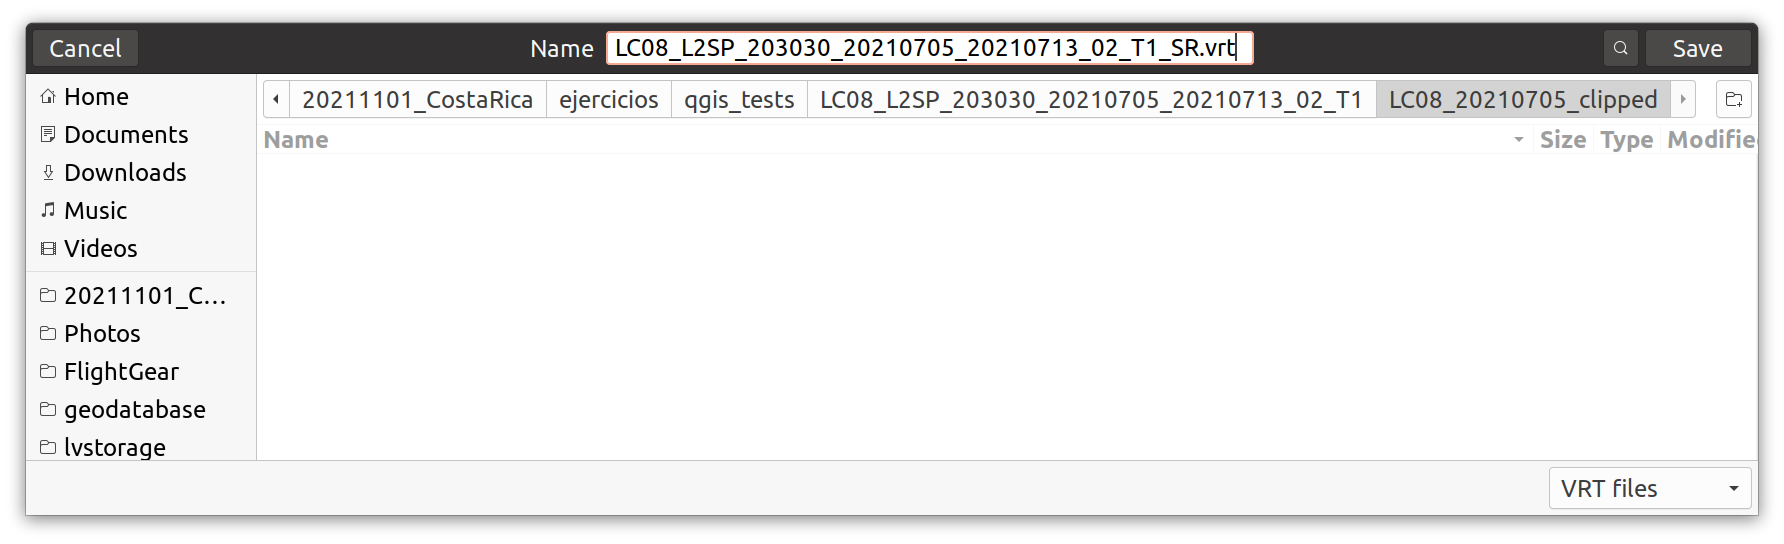
\includegraphics[width=\textwidth]{qgis_save_vrt}
       \end{figure} 
      \end{enumerate}

      El resultado final es una imagen con las 7 bandas espectrales de Landsat. Ahora puedes por ejemplo visualizar distintas combinaciones de color tal y como hicimos durante el curso básico de QGIS. Por ejemplo aquí tienes el resultado de una composición en falso color con el infrarrojo cercano (R: banda 5, G: banda 4 B: banda 3) del páramo de León (NW de España)
      
       \begin{figure}[H]\centering
        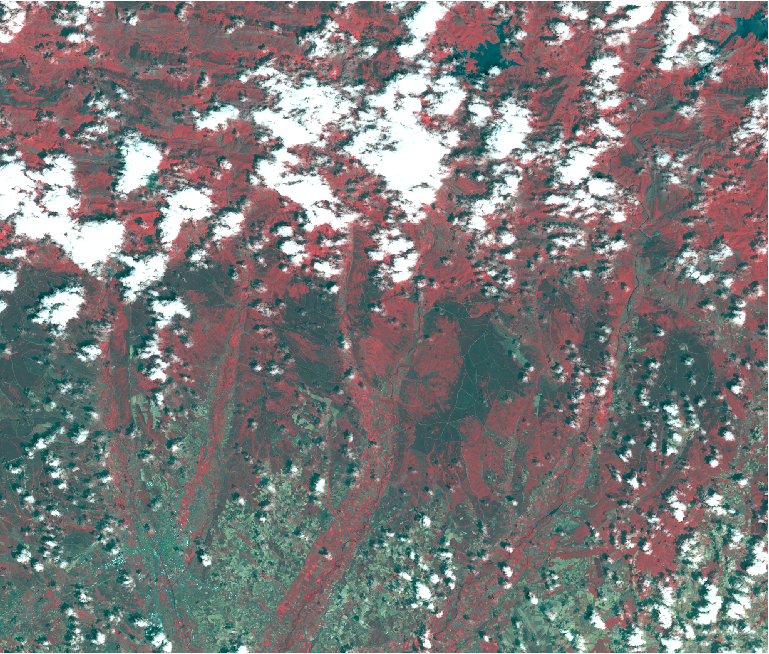
\includegraphics[width=\textwidth]{paramo_leon}
       \end{figure}
       
      Con esta imagen apilada, junto con la máscara de nubes e información adicional que sacaremos de los metadatos, podemos ya ejectuar nuestro algoritmo para derivar los parámetros biosfísicos:
      
      \begin{enumerate}
       \item De nuestra herramienta \cverb+Evapotranspiration Processor+, ejecuta la función \cverb+Biophysical Processor based on Pro4SAIL+, dentro del grupo \cverb+Land Surface Products+. 
       
       \begin{figure}[H]\centering
        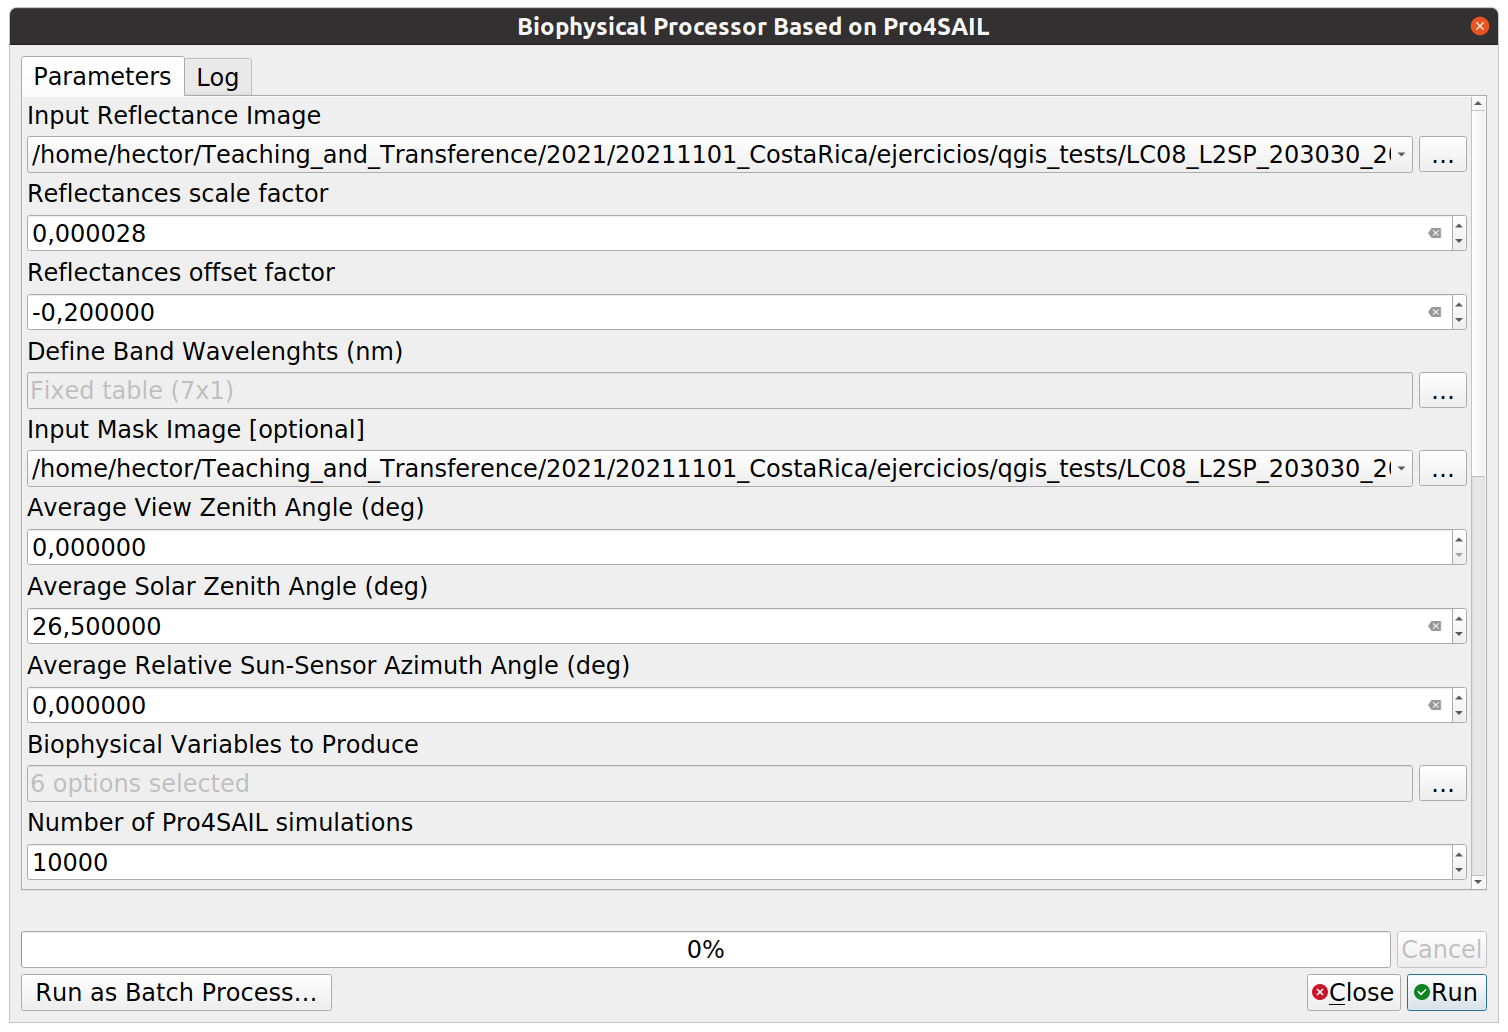
\includegraphics[width=\textwidth]{qgis_biophysical_processor}
       \end{figure}
       
       \item En \cverb+Input Reflectance Image+, selecciona nuestro ráster virtual apilado.
       
       \item En \cverb+Reflectances scale factor+ y \cverb+Reflectances offset factor+ tenemos que poner los factores de conversión de los valores digitales de la imagen a reflectividades (de manera análoga a lo que hicimos con la imagen de temperatura de superficie). Para ellos tenemos que abrir los metadatos de la imagen y buscar las líneas que comiencen por \cverb+REFLECTANCE_ADD_BAND+ y \cverb+REFLECTANCE_MULT_BAND+. Hay una línea por banda, pero verás que todas las bandas de reflectividad tienen los mismos valores para \cverb+ADD+ como para \cverb+MULT+. Anota o copia estos valores e introdúcelos en las casillas correspondientes de nuestra función.
       
       \item Ahora tenemos que decirle al algoritmo qué longitudes de onda representan cada banda. En \cverb+Define Band Wavelengths+ pincha en los tres puntitos y añade tantas filas como bandas tenga tu imagen (7 en este caso). En cada fila introduce la longitud de onda correspondiente al orden de las bandas. Como nosotros tenemos las siete bandas de Landsat 8 ordenadas de menor a mayor, los valores que habría que introducir son 440, 480, 560, 655, 865, 1610, 2200\footnote{Puedes ver las designaciones de las bandas de Landsat en esta dirección \url{https://www.usgs.gov/faqs/what-are-band-designations-landsat-satellites?qt-news_science_products=0#qt-news_science_products}. En nuestro caso tomamos el valor central o promedio de cada banda}.
       
       \begin{figure}[H]\centering
        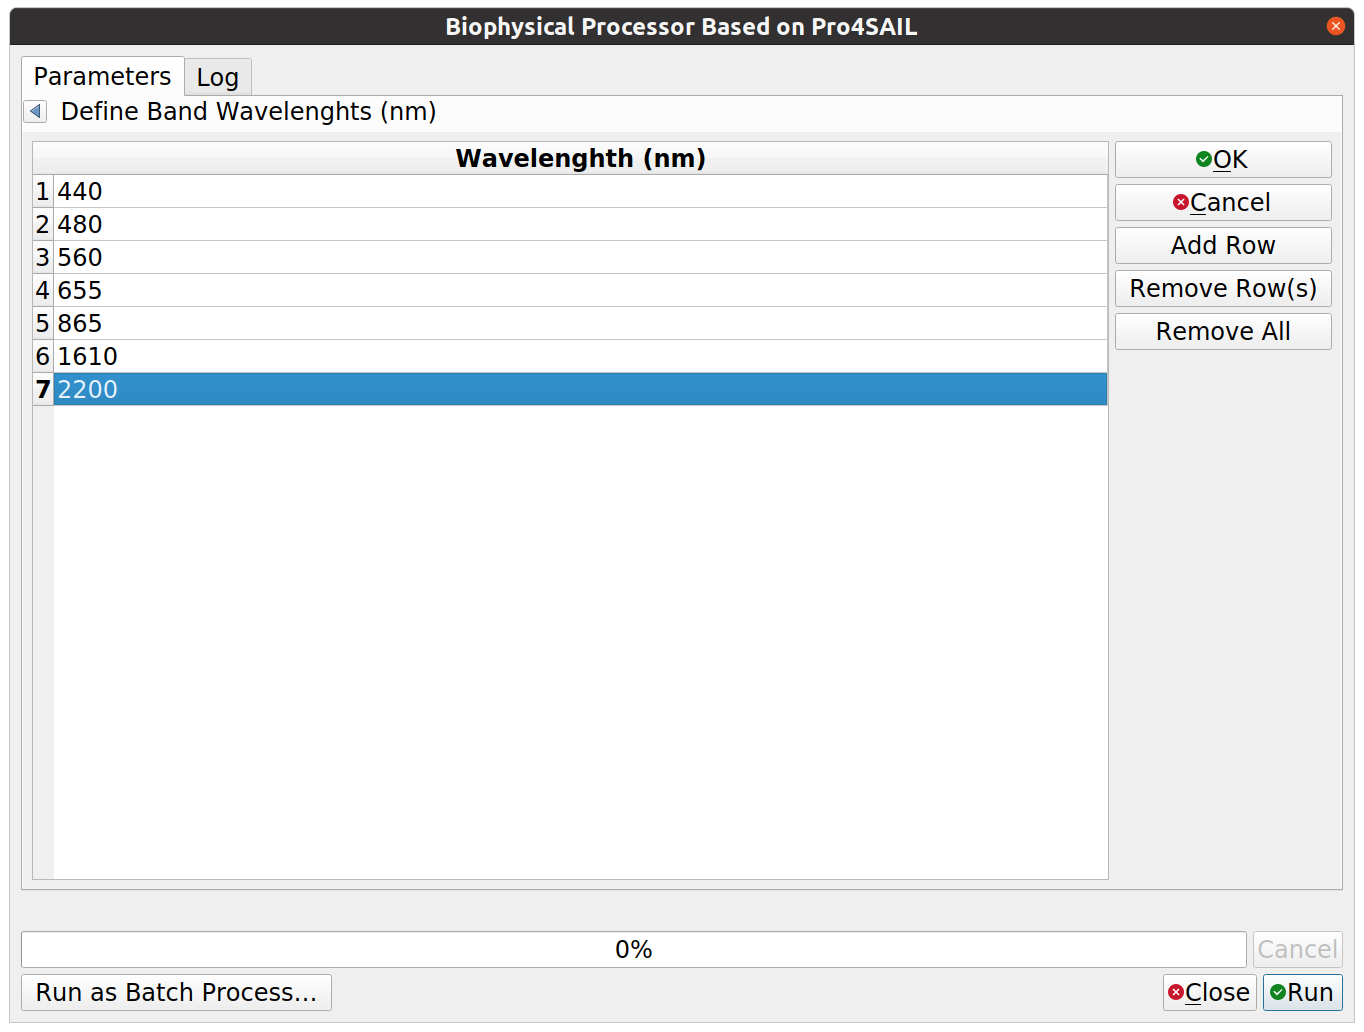
\includegraphics[width=\textwidth]{qgis_wl_input}
       \end{figure}
       
       \item En \cverb+Input Mask Image [Optional]+ selecciona la imagen de máscara de nubes que generamos anteriormente. Así sólo se realizarán los cálculos en los píxeles sin nubes ni sombras.
       
       \item Landsat tiene un ángulo de observación muy estrecho, y por tanto puedes dejar el valor 0 por defecto en \cverb+Average View Zenith Angle (deg)+.
       
       \item Busca en los metadatos de la imagen Landsat una línea que contenga el texto \cverb+SUN_ELEVATION+. Resta ese valor a 90 ($90 - SUN\_ELEVATION$) e introduce ese valor en \cverb+Average Solar Zenith Angle (deg)+.
       
       \item El ángulo azimutal relativo sol-sensor \\(\cverb+Average Relative Sun-Sensor Azimuth Angle (deg)+) sólo es relevante si el ángulo cenital de observación es distinto de 0, por lo que deja esta casilla con su valor por defecto.
       
       \item En \cverb+Biophysical Variables to Produce+ podemos elegir qué parámetros biosfísicos queremos generar. Selecciona al menos \cverb+Leaf Area Index+, \cverb+Leaf Chlorophyll+, \cverb+Leaf Water Content+, \cverb+Leaf Dry Matter Content+, \cverb+fraction of Absorbed PAR+ y \cverb+fraction of Intercepted PAR+.
       
       \begin{figure}[H]\centering
        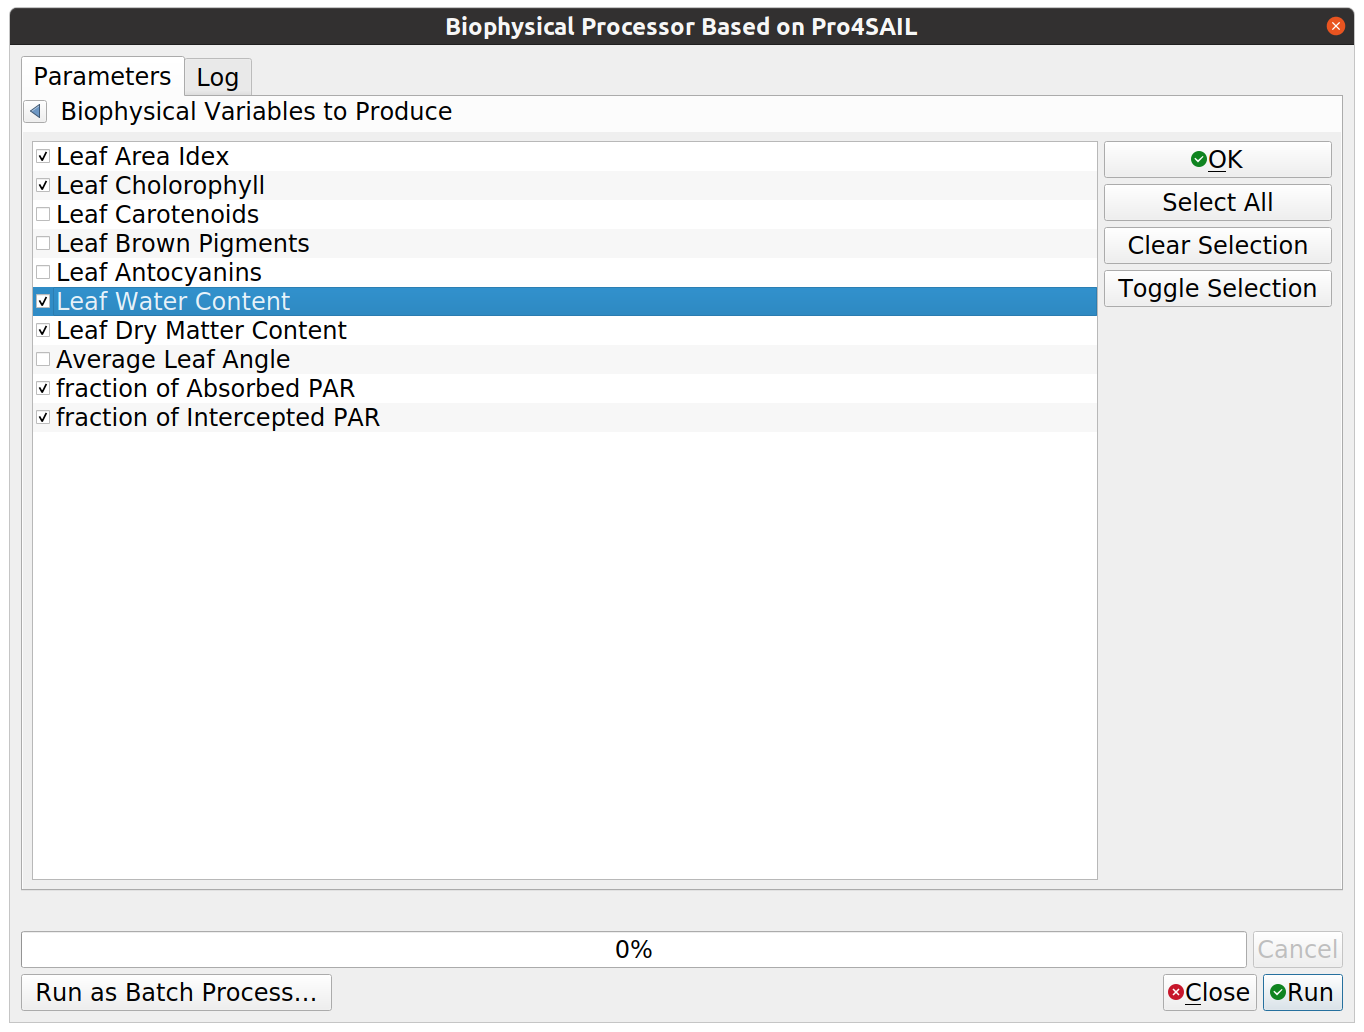
\includegraphics[width=\textwidth]{qgis_biophysical_selector}
       \end{figure}
      
       \item En \cverb+Number of Pro4SAIL simulations+, según la potencia de tu PC puedes aumentar o disminuir el número de simulaciones. Cuantas más simulaciones más robusta será la estimación, pero también tardará más tiempo en procesar e incluso puede que te quedes sin memoria RAM. 10000 simulaciones es un buen punto de partida.
      
       \item \cverb+Number of CPUS+ le dice al algoritmo cuantos procesos en paralelo quieres que haga. Cuantos más CPUs use más rápido serán los cálculos. El número máximo aconsejable es el número máximo de núcleos que tenga tu PC. Si lo desconoces, puedes dejar el valor a 0 y el algoritmo mismo contará los núcleos que tienes.
      
       \item El resto de las casillas determinan el rango de valores espaerables en tu zona o cultivo para cada una de las variables biofísicas\footnote{Como recordatorio puedes volver al ejercicio que realizamos en MyBinder ()\url{https://mybinder.org/v2/gh/hectornieto/Curso-WUE/HEAD})}. Si desconoces la variabilidad esperable puedes dejar los valores por defecto. 
      
       \item Finalmente selecciona la carpeta de salida donde se guardarán estos productos biofísicos. Puedes usar la carpeta donde tienes guardadas tus imágenes recortadas.
      \end{enumerate}
     
      El proceso tardará un rato, según la potencia de tu PC, el número de simulaciones que hayas solicitad y el tamaño de tu imagen recortada. Al final obtendrás una imagen por producto solicitado, el algoritmo utiliza automáticamente como nombre del archivo el nombre de la carpeta donde se guardan las imágenes, y cada imagen tiene un sufijo indicando el producto que representa: \cverb+CAB+ para la clorifila ($\mu g/cm^2$), \cverb+CAR+ para los carotenoides ($\mu g/cm^2$), \cverb+CBROWN+ para los pigmentos marrones (--), \cverb+ANT+ para los antocianinos ($\mu g/cm^2$), \cverb+CW+ para el contenido de agua de la hoja ($g/cm^2$), \cverb+CM+ para el peso específico de la hoja ($g/cm^2$), \cverb+LAI+ para el LAI, \cverb+LEAF_ANGLE+ para el ángulo de inclinación típico de las hojas (º), \cverb+FAPAR+ y \cverb+FIPAR+ para la fracción de radiación PAR absorbida e interceptada respectivamente.
     
    \subsubsection{Productos biofísicos adicionales}
      Desgraciadamente hay otros parámetros que no podemos estimar directamente con nuestros datos espectrales. Se trata de la información relativa a la arquitectura del dosel (altura y grado de agrupamiento). Si tu zona de interés es muy homogénea puedes asumir una altura de la vegetación constante, pero lo normal es que en tu región se encuentren varios tipos de cobertura e incluso distintos cultivos. Es por ello que en esta práctica estos parámetros los vamos a determinar en función de un mapa de tipos de cobertura. Podremos usar un mapa de cobertura generado por todo el Globo a 100m de resolución, dentro del servicio Copernicus, pero igualmente si dispones de un mapa de cultivos, de usos de suelo o de aprovechamientos de tu zona puedes usarlo en su lugar, y saltarte estos tres pasos:
      
      \begin{enumerate}
       \item Accede a este servicio de Copernicus (no requiere registro previo) \url{https://lcviewer.vito.be} y en la esquina superior derecha pincha en \cverb+Download+
       \begin{figure}[H]\centering
        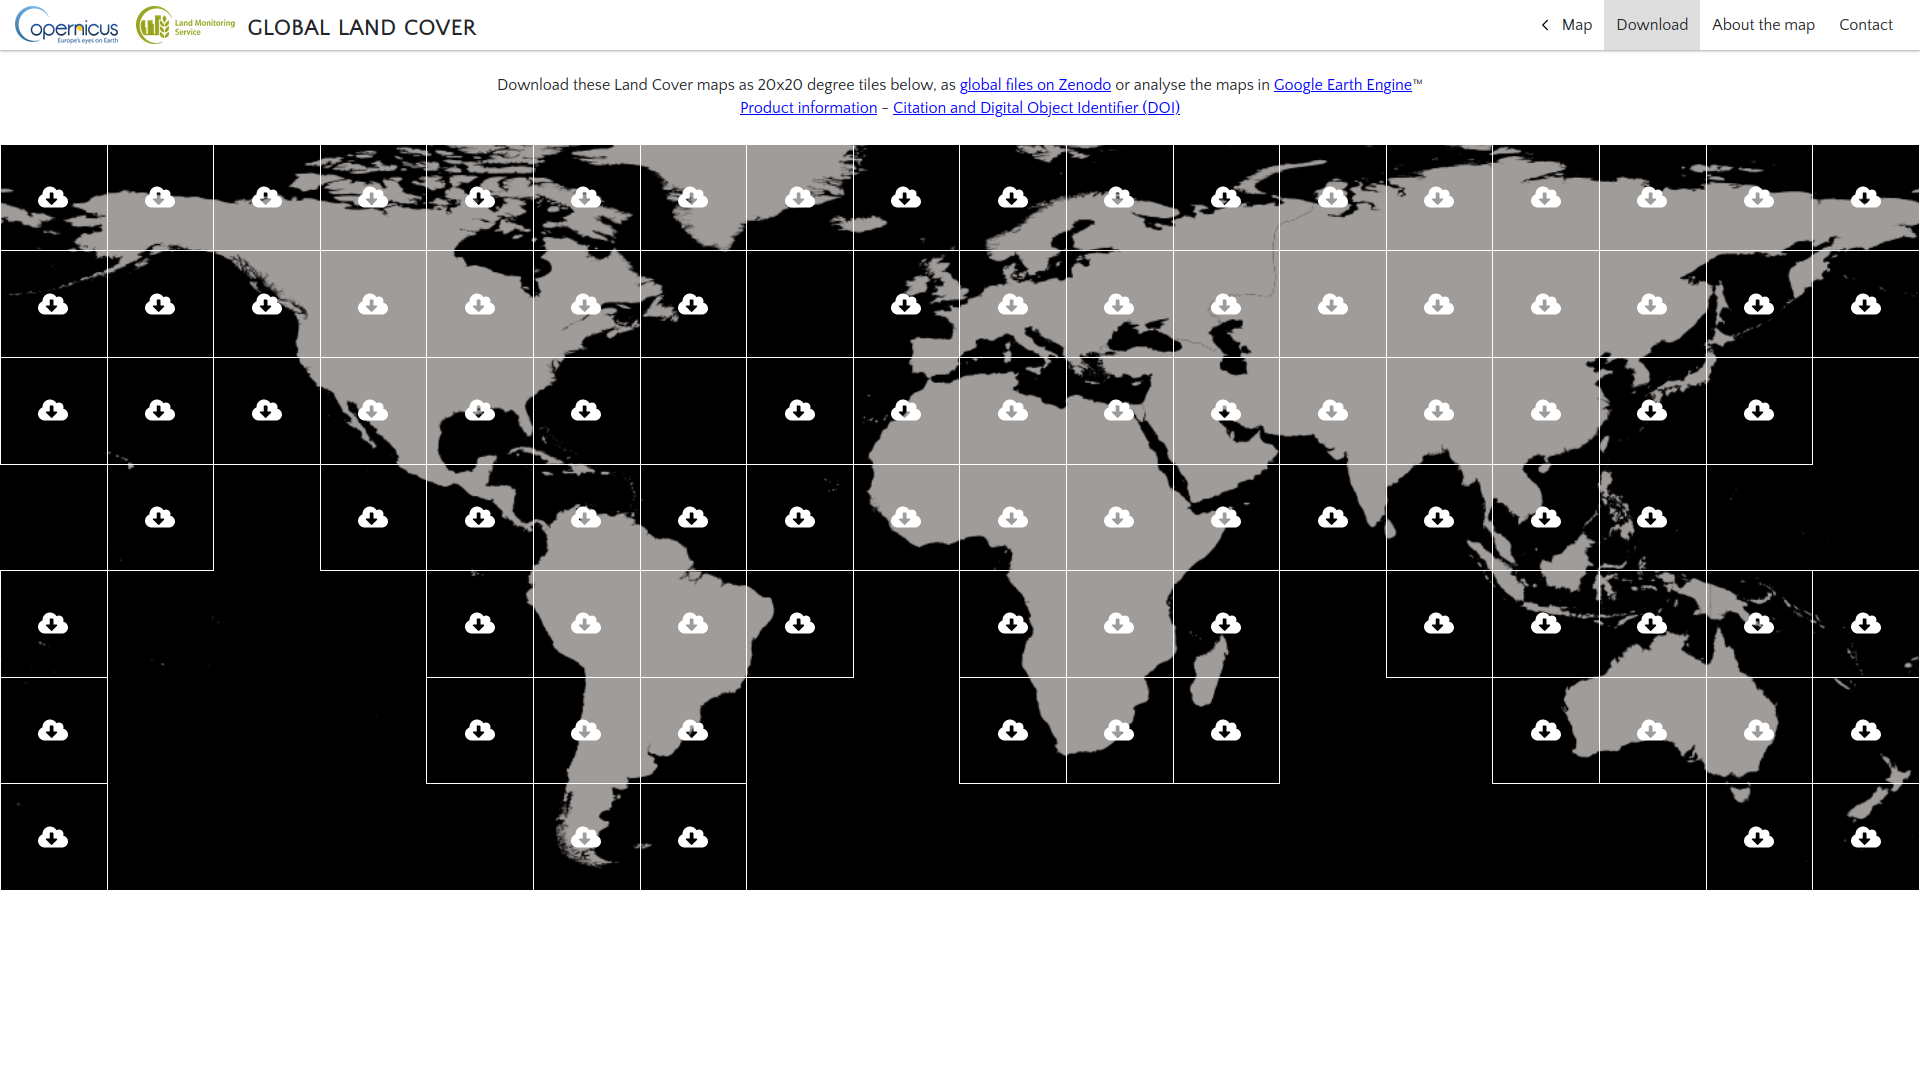
\includegraphics[width=\textwidth]{clc_web}
       \end{figure}
       
       \item Pincha en el mapa de la Tierra la tesela donde se encuentra tu zona de estudio, y aparecerá este cuadro de diálogo.
       \begin{figure}[H]\centering
        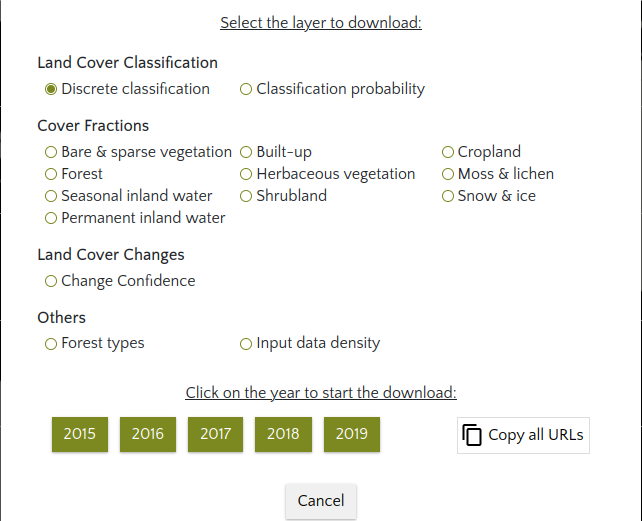
\includegraphics[width=\textwidth]{clc_download_options}
       \end{figure}
       \item Deja seleccionado \cverb+Discrete classification+ y selecciona el año de interés para empezar la descarga del mapa\footnote{El año más reciente es de momento 2019, para años más recientes usa 2019 asumiendo que las coberturas del suelo no han cambiado significativamene entre años}. Guárdalo donde desees.
      \end{enumerate}
      
      Abre el mapa en QGIS. Verás que el mapa descargado ocupa seguramente una región mucho más amplia que nuestra zona de estudio, tiene una resolución de 100m y está en coordenadas geográficas. Por otro lado aún tenemos que asignar valores de altura y cobertura del suelo en función del tipo de cubierta. Como un raster es una matriz de números, verás además que cada cobertura está asociado a un valor numérico (su ID). 
      
      El material de la práctica de hoy incluye una tabla en formato \cverb+.csv+ (\cverb+CopernicusLandCover_conversion.csv+) con las conversiones de los tipos de vegetación del mapa de cobertura a los valores de altura del dosel, fracción ocupada por el suelo, y tamaño típico de la hoja. Puedes abrir esta tabla como una hoja de cálculo (p.ej. en Excel o LibreOffice). Verás que hay una línea por cada \cverb+ID+ del mapa de clasificación. Puedes editar los valores de las columnas \cverb+Altura Dosel (m)+, \cverb+Fracción ocupada del suelo+ y \cverb+Tamaño de la hoja/foliolo+. El tamaño de la hoja, o del foliolo en caso de hojas compuestas, no es tan importante por lo que si tienes dudas en asignar un valor típico mantén los valores por defecto. 
      
      \begin{table}[H]
      \centering
      \footnotesize
       \begin{tabular}{lp{5cm}b{1.2cm}b{1.2cm}b{1.2cm}}
       \toprule
        ID& Tipo& Altura Dosel (m)& Fracción ocupada del suelo& Tamaño de la hoja o foliolo\\
        \midrule
        20& Matorral& 2.00& 1.00& 0.05\\
        30& Pastizal& 1.00& 1.00& 0.02\\
        40& Cultivo& 1.5& 1.00& 0.02\\
        41& Cultivo, secano& 1.5& 1.00& 0.02\\
        42& Cultivo, regadío& 1.5& 1.00& 0.02\\
        43& Cultivo, barbecho& 0.5& 1.00& 0.01\\
        50& Urbano& 30.00& 0.00& 0.00\\
        60& Suelo desnudo& 0.00& 0.00& 0.00\\
        70& Nieve/hielo permanente& 0.00& 0.00& 0.00\\
        80& Agua& 0.00& 0.00& 0.00\\
        81& Agua: temporal& 0.00& 0.00& 0.00\\
        90& Matorral o herbáceas inundadas& 2.00& 1.00& 0.1\\
        100& Musgos y líquenes& 0.3& 1.00& 5.00\\
        111& Bosque: coníferas perennes, bosque cerrado ($>$40\%)& 10.00& 0.8& 0.05\\
        112& Bosque: frondosas perennes, bosque cerrado ($>$40\%)& 5.00& 0.8& 0.15\\
        113& Bosque: coníferas caducas, bosque cerrado ($>$40\%)& 10.00& 0.8& 0.05\\
        114& Bosque: frondosas caducas, bosque cerrado ($>$40\%) & 8.00& 0.8& 0.15\\
        115& Bosque: mixto cerrado& 8.00& 0.8& 0.1\\
        116& Bosque: tipo desconocido cerrado& 5.00& 0.8& 0.1\\
        121& Bosque: coníferas perennes, bosque abierto (15 - 40\%)& 5.00& 0.3& 0.05\\
        122& Bosque: frondosas perennes, bosque abierto (15 - 40\%)& 4.00& 0.3& 0.15\\
        123& Bosque: coníferas caducas, bosque abierto (15 - 40\%)& 5.00& 0.3& 0.05\\
        124& Bosque: frondosas caducas, bosque abierto (15 - 40\%)& 4.00& 0.3& 0.15\\
        125& Bosque: mixto abierto (15 - 40\%)& 5.00& 0.3& 0.1\\
        126& Bosque: tipo desconocido abierto & 3.00& 0.3& 0.1\\
        200& Aguas costeras& 0.00& 0.00& 0.00\\
        0& No válido& 0.00& 0.00& 0.00\\
        \bottomrule
       \end{tabular}
      \end{table}

      Si dispones de un mapa de cultivos y usos del suelo más detallado puedes usarlo para esta práctica, tan sólo tendrías que generar una tabla similar relacionando los tipos de cultivo con sus alturas, fracción ocupada del suelo si éste es un cultivo en hilera o con un marco de plantación evidente, y el tamaño típico de la hoja.
      
      Una vez que hayas editado y adaptado la tabla guárdala en formato csv, mejor como una copia de la original. En primer lugar vamos a reclasificar el mapa para obtener de él los valores que nos interesan.
            
      \begin{enumerate}
       \item Abre la tabla en QGIS, para ello abre el \cverb+Administrador de fuentes de datos+ y selecciona la opción \cverb+Texto delimitado+\footnote{Delimited text}.
       \begin{figure}[H]\centering
        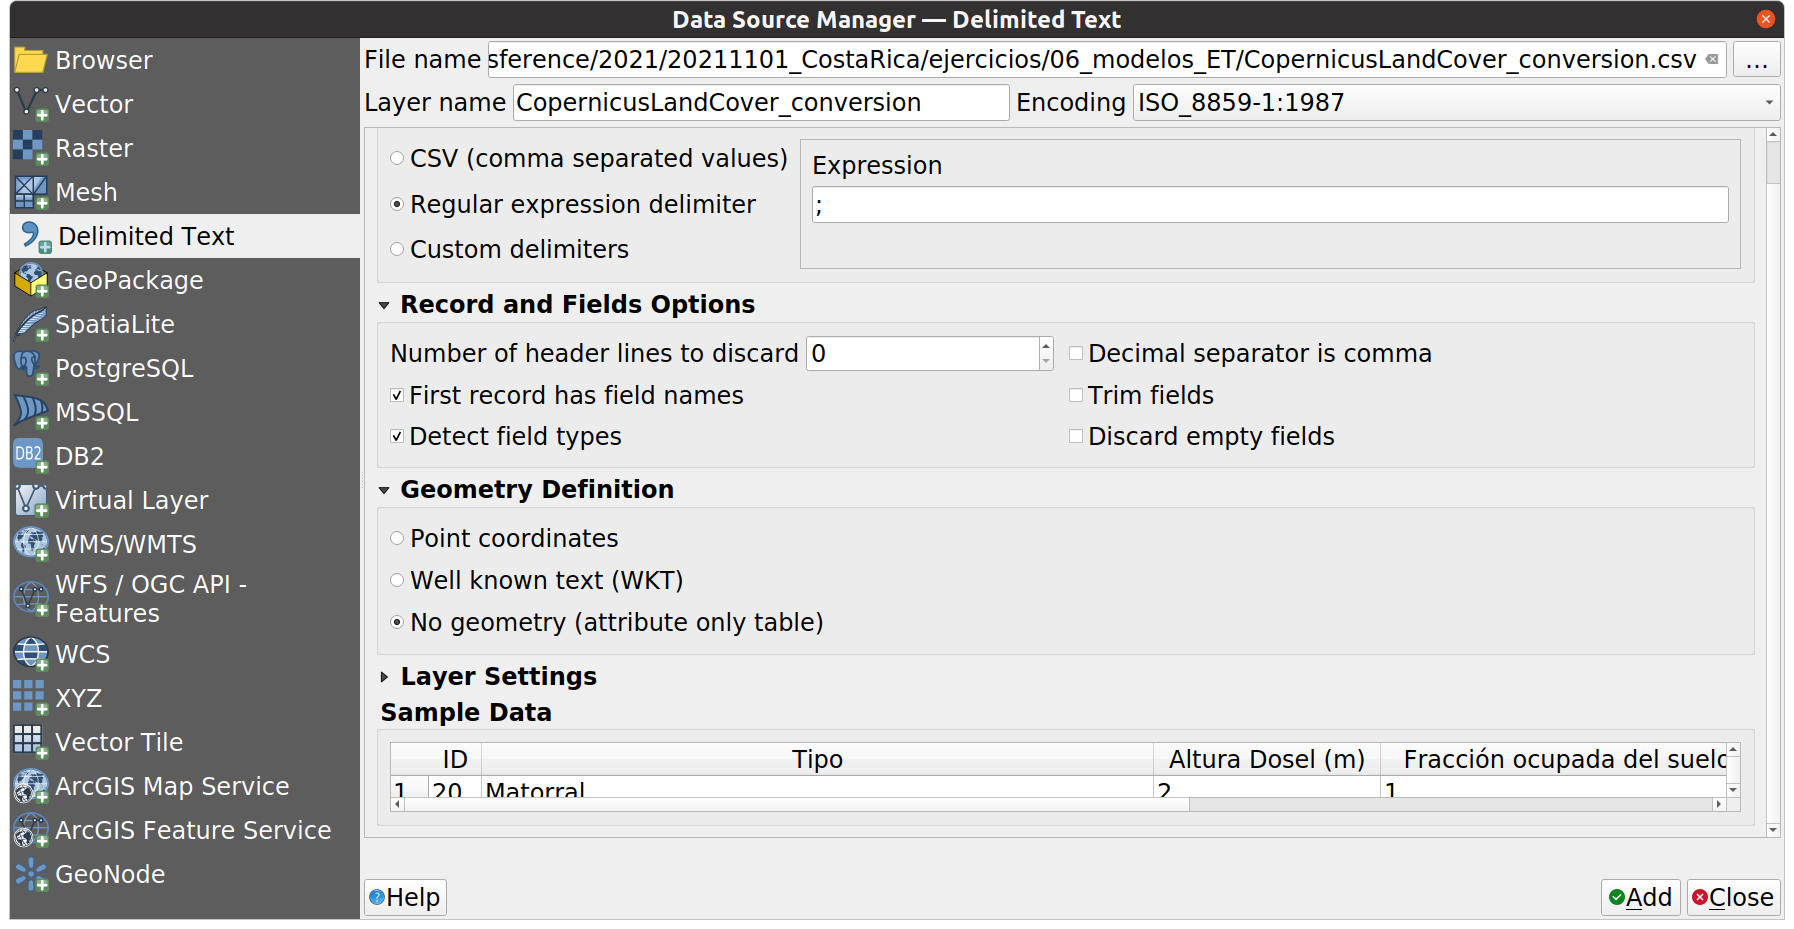
\includegraphics[width=\textwidth]{qgis_delimited_text}
       \end{figure}
       
       \item En \cverb+Nombre de archivo+\footnote{File name} selecciona la tabla \cverb+csv+.
       
       \item Selecciona \cverb+Delimitador de expresión regular+\footnote{Regular expression delimiter} y en la casilla pon \cverb+;+, ya que en nuestra tabla csv los campos están delimitados por punto y coma.
       
       \item En \cverb+Definición de geometría+\footnote{Geometry definition} selecciona\\
       \cverb+Ninguna geometría (tabla sólo de atributos)+\footnote{No geometry (attribute only table)}.
       
       \item Deja el resto de las opciones por defecto, comprueba en la zona de datos de ejemplo que las filas y columnas de nuestra tabla son interpretadas correctamente por el software, y presiona \cverb+Añadir+\footnote{Add} para añadir la tabla a nuestro entorno QGIS.
      
       Verás que la tabla aparece en el gestor de capas de QGIS, pero aún sólo es una tabla, por lo que aún no tiene una representación espacial. 
       \begin{figure}[H]\centering
        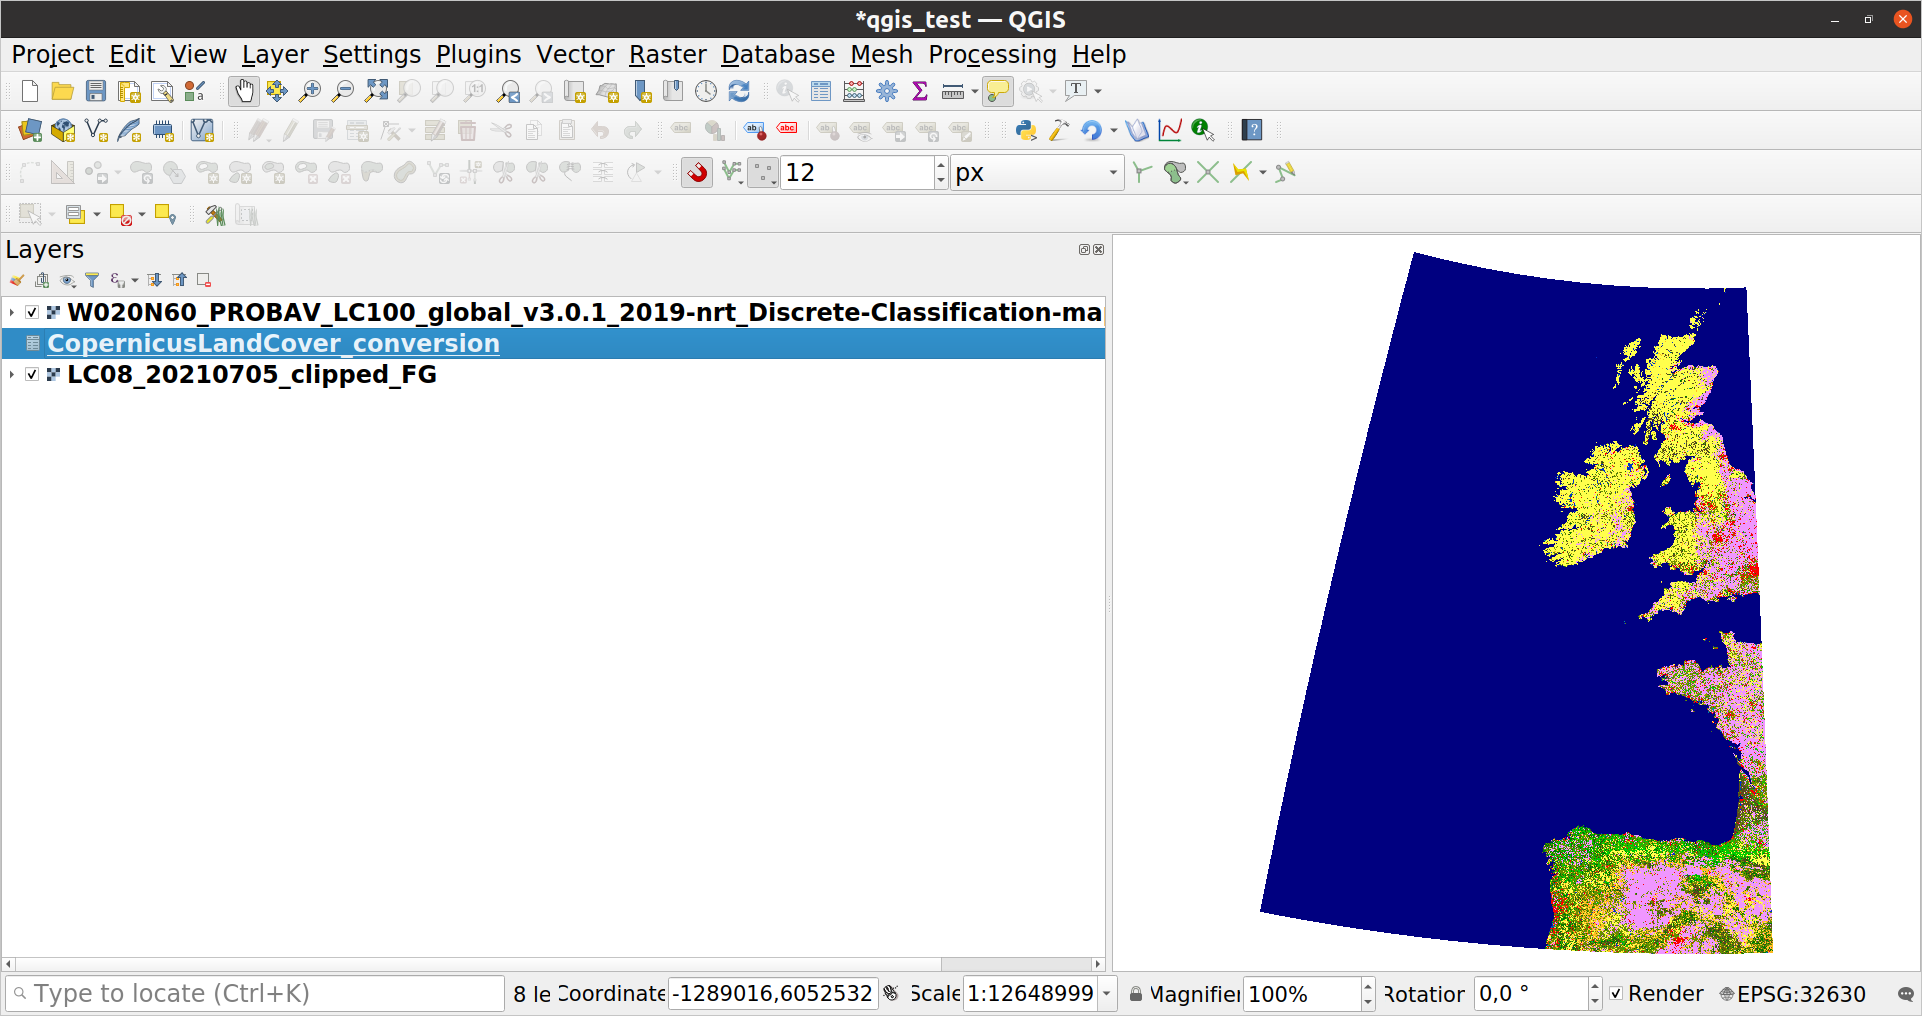
\includegraphics[width=\textwidth]{qgis_open_csv}
       \end{figure}
      
       \item Ejecuta ahora la función \cverb+Reclasificar por capa+\footnote{Reclasify by layer} dentro de \cverb+Análisis ráster+\footnote{Raster analysis} en la caja de herramientas.
      
       \begin{figure}[H]\centering
        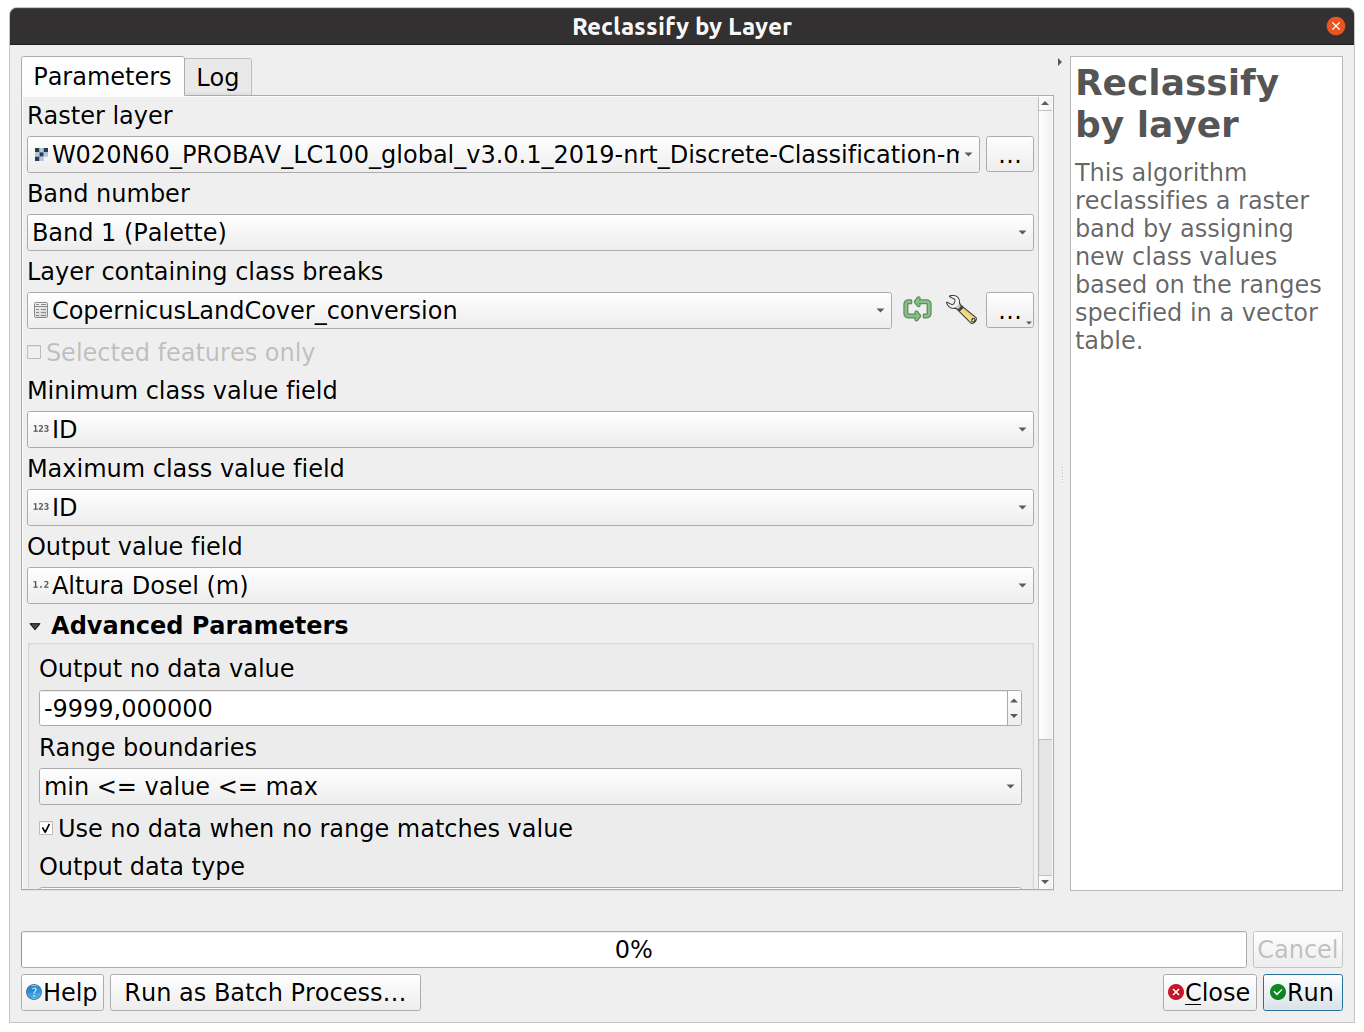
\includegraphics[width=\textwidth]{qgis_reclasify_raster}
       \end{figure}
       
       \item Selecciona tu mapa de tipos de cobertura en \cverb+Capa ráster+\footnote{Raster layer+}
       
       \item En \cverb+Capa que contiene saltos de clase+\footnote{Raster containing class breaks} selecciona la tabla que acabamos de generar y abrir en QGIS.
       
       \item Tanto en \cverb+Campo de valor de clase mínimo+\footnote{Minimum class value field} como en\\
       \cverb+Campo de valor de clase máximo+\footnote{Maximum class value field} selecciona la columna \cverb+ID+
      
       \item Elige la columna \cverb+Altura Dosel (m)+ en \cverb+Campo de valor de salida+\footnote{Output value field} con el fin de generar el mapa de alturas de dosel.
      
       \item Dentro de \cverb+Parámetros avanzados+\footnote{Advanced parameters} selecciona \cverb+min <= value <= max+ para \cverb+Límites de rango+\footnote{Range boundaries}. Al seleccionar el ID como criterio mínimo y máximo junto con esta selección de límites de rango nos aseguramos que el algoritmo asigna correctamente el valor de altura según el ID único del mapa de tipos de cobertura.
      
       También marca la opción \cverb+No usar datos cuando ningún rango coincide con el valor+\footnote{Use no data when no range matches value}.
      
       \item Finalmente selecciona una imagen de salida en \footnote{Reclassified raster} y ejecuta la función.
      
       \item Repite los mismos pasos para generar también el mapa de fracción ocupada del suelo y tamaño de la hoja asignando en \cverb+Campo de valor de salida+\footnote{Output value field} la columna correspondiente.
      \end{enumerate}
      
      Ahora tenemos tres nuevos mapas, lo último que tenemos que hacer es alinear estos tres mapas para que solapen con la extensión y resolucińo de nuestros inputs. Para ello vuelve a ejecutar la función \cverb+Match image geometry+ del complemento \cverb+Evapotranspiration Processor+. Como siempre, selecciona la temperatura de superficie recortada a tu zona de estudio como imagen de referencia, elige los tres nuevos mapas generados, y selecciona \cverb+Bilinear+ como método de remuestreo.
  
\section{{[Opcional]} Descripción del modelo TSEB}
  El modelo TSEB (Two-Source Energy Balance) es un modelo de balance energético de dos fuentes, es decir separa los flujos de calor y vapor de agua entre la vegetación y el suelo. Por tanto el modelo permite estimar y separar la transpiración de la planta de la evaporación del suelo.
  
  La variable fundamental de entrada es la temperatura radiométrica de la superficie, que medimos con nuestro sensor de teledetección. La principal característica de TSEB frente a otros modelos es que éste permite explicar e integrar la variabilidad angular presente en la temperatura de la superficie medidad por el sensor, según el ángulo de observación, separando esta información radiométrica en una temperatura de hoja y una temperatura de suelo.
  
  \begin{figure}[H]\centering
   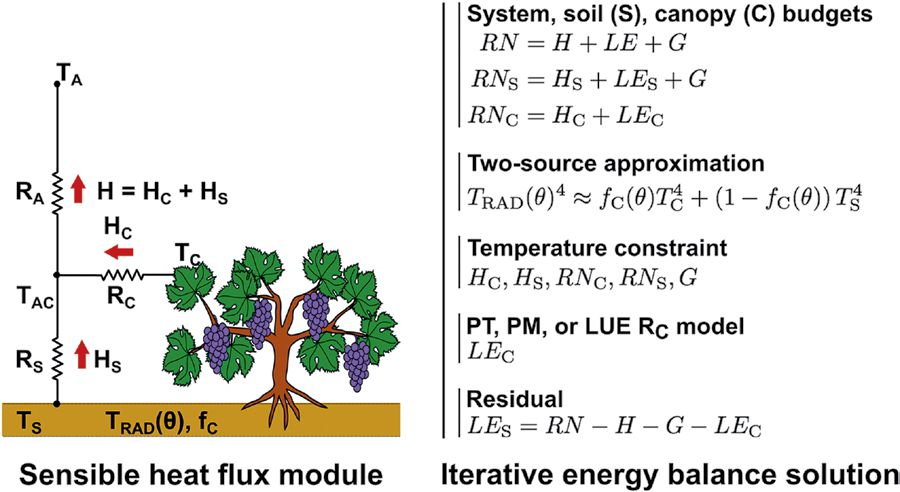
\includegraphics[width=\textwidth]{tseb_scheme}
  \end{figure}
  
  Como la mayoría de los modelos de Evapotranspiración basados en la temperatura de la superficie, la ET, o flujo de calor latente ($\lambda E$), se estima como residuo de las otras componentes del balance energético (Eq. \ref{eq:Energy_Balance})
  
  \begin{subequations}\label{eq:Energy_Balance}
   \begin{align}
    R_{n} & \approx H + \lambda E + G\\
    R_{n,S} & \approx H_{S} + \lambda E_{S} + G\\
    R_{n,C} & \approx H_{C} + \lambda E_{C}\label{eq:Energy_Balance_TSEB}
   \end{align}
  \end{subequations}
  $R_n$ es la radiación neta (W/m²), $H$ el flujo de calor sensible, y $G$ es el flujo de calor almacenado en el suelo (todos los flujos expresados en W/m²). El símbolo ``$\approx$'' aparece ya que hay componentes del balance energético que generalmente se consideran despreciables, como puede ser el transporte de calor lateral o advección, el almacenamiento de calor en la vegetación, o la energía usada durante la fotosíntesis para fijar el CO$_2$.
  
  $R_{n,C}$ y $R_{n,S}$ se estiman a partir de un modelo simplificado de transferencia radiativa en el que como variables de entrada, a parte de la irradiancia, están en índice de área foliar ($LAI$), la distribución angular de las hojas, la absortividad de la hoja y la reflectividad del suelo. Además, el modelo al simular la transmisión y absorción de luz solar en doseles horizontalmente heterogéneos (cultivos en hilera o copas aisladas) considera un grado de acomplamiento de las hojas basado en la fracción de cobertura del dosel ($f_c$).
  
  $G$ suele estimarse en las horas centrales del día como una fracción de la radiación neta del suelo ($G = 0.35R_{n,S}$). Por otro lado $H_C$ y $H_S$ se calculan como:
  
  \begin{equation}\label{eq:H_partition}
   \begin{aligned}
    H=H_{C}+H_{S}=&\rho_{air} C_{p}\frac{T_{0}-T_{A}}{R_{a}}\\
    =&\rho_{air} C_{p}\left[\frac{T_{C}-T_{0}}{R_{x}}+\frac{T_{S}-T_{0}}{R_{s}}\right]
   \end{aligned}
  \end{equation}
  donde $\rho_{air}$ es la densidad del aire (kg/m³), $C_{p}$ es la capacidad calorífica del aire a presión constante  (J/kg/K) , $T_{0}$ es la temperatura aerodinámica, estimada como $T_{AC}=\frac{\frac{T_A}{R_a}+\frac{T_C}{R_x}+\frac{T_S}{R_s}}{\frac{1}{R_a} +\frac{1}{R_x}+\frac{1}{R_s}}$. $R_{a}$ es la resistencia aerodinámica al transporte de calor (s/m), $R_{s}$ es la resistencia al tranporte de calor entre el suelo y el aire (s/m), y $R_{x}$ es la resistencia al transporte de calor del dosel vegetal (s/m):

  \begin{subequations}
   \label{eq:resistances_series}
   \begin{align}
    R_{a}&=\frac{\ln\left(\frac{z_{T}-d_0}{z_{0H}}\right)-\Psi_{h}\left(\frac{z_{T}-d_0} {L}\right)+\Psi_{h}\left(\frac{z_{0H}}{L}\right)}{\kappa '\,u_{*}}\label{eq:ra}\\
    R_{s}&=\frac{1}{c\left(T_{S}-T_{A}\right)^{1/3}+b\,u_{s}}\label{eq:rs}\\ 
    R_{x}&=\frac{C'}{\mathrm{LAI}}\left(\frac{l_w}{u_{d_0+z_{0M}}}\right)^{1/2}\label{eq:rx}
   \end{align}
  \end{subequations}
  $u_s$ y $u_{d_0+z_{0M}}$ son las velocidades del viento en las proximidades del suelo y dentro del dosel vegetal respetivamente. $l_w$ es el tamaño típico de la hoja (m), y $b=0.0038$, $c=0.012$ y $C'=90$ son constantes. $u_{*}$ es la velocidad de fricción (m/d) calculada como

  \begin{equation}\label{eq:u_friction}
   u_{*}=\frac{\kappa '\,u}{\left[\ln\left(\frac{z_{u}-d_0}{z_{0M}}\right)-\Psi_{m} \left(\frac{z_{u}-d_0}{L}\right)+\Psi_m\left(\frac{z_{0M}}{L}\right)\right]}
  \end{equation}

  En la ecuación \ref{eq:u_friction} $z_{u}$ y $z_{T}$ son las alturas sobre el terreno a las que se realizan las mediciones de la velocidad del viento, $u$ (m/s), y la temperatura del aire, $T_{A}$ (K). $d_0$, $z_{0M}$ y $z_{0H}$ son los coeficientes de rugosidad aerodinámica de la superficie (m), estimados a partir de la altura de la vegetación ($h_C$, m). En TSEB $z_{0H}$ se asume igual a $z_{0M}$ ya que el término $R_x$ ya considera la diferencia de eficiencia del transporte de calor con respecto al transporte de aire. $\kappa '=0.4$ is la constante de von Karman. Los coeficientes $\Psi_{m}\left(\zeta\right)$ y $\Psi_{h}\left(\zeta\right)$ de las ecuaciones \ref{eq:ra} y \ref{eq:u_friction} son los correctores adiabáticos por transporte convectivo. Estas dos variables por tanto dependen de la estabilidad atmosférica, que suele expresarse mediante la longitud de Monin-Obukhov, $L$ (m).

  \begin{equation}\label{eq:MO}
   L=\frac{-u_{*}^{3}\rho_{air}}{k\,g\left[^H/_{\left(T_{A}C_{p}\right)} +0.61E\right]}
  \end{equation}
  $E$ es la tasa de evaporación (kg/s), y $g$ es la aceleración de la gravedad (m/s)

  La clave de TSEB es la necesidad de obtener las temperaturas de hoja y suelo para así poder calcular $H_C$ y $H_S$, teniendo en cuenta que casi siempre la señal radiométrica de un píxel es una mezcla de vegetación y suelo. Esta temperatura de superficie medida por el sensor ($T_{rad}\left(\theta\right)$) puede descomponerse entre la radiación térmica emitida por las hojas y la emitida por el suelo, según la proporción de vegetación de hoja y suelo que capta el sensor, según el ángulo de observación del mismo ($\theta$):

  \begin{equation}\label{eq:TSEB_Trad}
   T_{rad}^4\left(\theta\right)=\left[1-P_{gap}\left(\theta\right)\right]T_{C}^4 + P_{gap}\left(\theta\right)T_{S}^4
  \end{equation}
  donde $P_{gap}\left(\theta\right)$ es la fracción de huecos de la vegetación en la dirección de observación del sensor. El problema reside que la ecuación \ref{eq:TSEB_Trad} contiene dos incógnitas ($T_C$ y $T_S$) para una única ecuación.
  
  TSEB intenta resolver problema mediante un proceso iterativo en que secuencialmente va buscando valores de $H_C$, $T_C$, $T_S$ and $H_S$. Este proceso iterativo comienza por un valor inicial de temperatura de la hoja, tras asumir que la planta transpira a su tasa potencial. Esta transpiración inicial puede estimarse de distintas maneras (modelos de Priestley-Taylor, Penman-Monteith, Shuttleworth-Wallace, ...) pero básicamente depende de la radiación absorbida por la planta ($R_{n,C}$) y la fracción de la planta que es verde y por tanto fotosintéticamente activa ($f_g$).
  
  Con esta transpiración incial podemos estimar un primer valor de $H_C$ y por tanto una estimación incial de $T_{C}$. $T_{S}$ puede entonces calcularse a partir de la ecuación \ref{eq:TSEB_Trad} y así hacer una primera estimación de los flujos de calor sensible ($H$) y latente del suelo ($\lambda E_S$). Llegados a este punto, es probable $\lambda E_S$ resulte en valores negativos, lo cual no es físicamente posible en las horas centrales del día ya que indicaría condensación en el suelo. Si esto ocurre es porque la transpiración inicial (asumida potencial) está sobre estimada, indicando además cierto nivel de estrés hídrico. Por tanto, el modelo, automáticamente y de manera secuencial, va reduciendo los valores de transpiración y recalculando todas las componentes del balance energético hasta que se obtenga una solución físicamente posible, esto es, flujos latentes positivos o nulos. Una vez que se logra una solución físicamente plausible el modelo detiene este proceso iterativo, obteniéndose las estimaciones finales de $H_C$, $LE_C$, $H_S$ y $LE_S$.
  
  \subsection{Extrapolación a ET diaria}
   Los flujos de calor y agua estimados por el modelo TSEB son los correspondientes al momento de adquisición de la temperatura radiométrica, es decir a la hora de pasada del satélite o del vuelo UAV. Además estos flujos vienen expresados en términos de energía (W/m²). Esta información puede ser muy útil para estudios meteorológicos o simplemente para validar estos flujos con las estimaciones de las estaciones de covarianza de flujos. Sin embargo, desde un punto de vista agronómico nos interesa y nos es más fácil trabajar con datos de ET diarios y expresados en unidades de masa (mm/día). 
   
   El flujo latente diario ($\lambda E_{day}$) se estima a partir de estas métricas instantáneas asumiendo que la proporción entre el flujo de agua ($\lambda E$) y la irradiancia solar ($S^\downarrow$) se mantiene constante a lo largo del día, de modo que:
    
   \begin{equation}\label{eq:et}
    \lambda E_{day} = S^\downarrow_{day} \frac{\lambda E_{i}}{S^\downarrow_{i}}
   \end{equation}
   donde $\lambda E_{i}$ y $S^\downarrow_{i}$ es el flujo de calor latente y la irradiancia solar instantáneos, en el momento de adquisición de la imagen, y $S^\downarrow_{day}$ es la irradiancia solar diaria.
   
   Finalmente el flujo de calor latente (W/m²) es convertido a ET (mm/día) mediante la siguiente ecuación:
   
    \begin{equation}\label{eq:et}
    ET_{day} = \frac{\lambda E_{day}}{\rho_w \lambda} \cdot 3600 \cdot 24 \times 10^3
   \end{equation}
   donde $\lambda$ es el calor latente de vaporización ($\lambda = 10^6 \times \{2.501 - \left[2.361 \times 10^{-3} \left(T_{air} - 273.15\right)\right]\}$, J/kg), $\rho_w$ es la densidad del agua ($\approx$1000 kg/m³), $3600 \cdot 24$ son los segundos que tiene un día y el factor $10^3$ convierte los metros en milímetros (mm/día).
   
 \section{Uso del modelo TSEB}
  \subsection{Imágenes Landsat}
   Partimos de tener los datos biofísicos procesados y con la extensión de nuestro mapa de temperatura, y los datos meteorológicos descargados y pre-procesados por la función \cverb+Retrieve meteorological variables from ECMWF+. Antes de ejecutar el modelo tenemos que asegurarnos que los datos meteo se ajustan también a nuestra imagen de temperatura de superficie. Originalmente los datos fueron descargados y procesados en función del MDT, por lo que es posible que la resolución y la extensión sean ligeramente distintas a nuestros datos térmicos. Es por ello que vamos a asegurarnos y alinear los datos meteorológicos al resto de datos de entrada.
   
   \begin{enumerate}
    \item Ejecuta la función \cverb+Match image geometry+
    
    \item Selecciona la imagen de temperatura como referencia
    
    \item selecciona como capas a remuestrear al menos las siguientes variables meteorológicas que necesita TSEB:
    
    \begin{itemize} 
     \item \cverb+TA+, temperatura del aire (K)
     \item \cverb+EA+, presión de vapor (mb)
     \item \cverb+P+, presión atmosférica (mb)
     \item \cverb+U+, velocidad del viento (mb)
     \item \cverb+SDN+, irradiancia solar (W/m²)
     \item \cverb+SDNDAY+, irradiancia solar diaria (W/m²)
     \item \cverb+ETREF+, ET de referencia diaria (mm/día)
    \end{itemize}
    
    \item Selecciona el método \cverb+Bilinear+ de remuestreo
    
    \item Selecciona una carpeta de salida
   \end{enumerate}

   \subsection{Preparación de la irradiancia de onda larga}
    El último parámetro que necesitamos es la irradiance de onda larga. Este parámetro no se encuentra procesado por la herramienta\\
    \cverb+Retrieve meteorological variables from ECMWF+. En cambio vamos a tener que calcularlo por nuestra cuenta.
    
    La irradiancia de onda larga depende principalmente de la temperatura y emisividad atmosféricas. Aplicando la ley de Stefan-Boltzman:
    \begin{equation*}
     L\downarrow = \sigma \epsilon_{atm} T_{air}^4
    \end{equation*}
    
    $\sigma$ es la constante de Stefan-Bolztman ($5.670374419...\times10^{-8}$ W/m²/K⁴), $T_{air}$ es la temperatura atmosférica en Kelvin y $\epsilon_{atm}$ es la emisividad atmosférica. Esta última depende principalmente de la humedad atmosférica, y puede estimarse como:
    
    \begin{equation*}
     \epsilon_{atm} = 1.24 \left[\frac{e_a}{T_{air}}\right]^{1/7}
    \end{equation*}
    siendo $e_a$ la presión de vapor atmosférica en mb.
    
    Tanto $T_{air}$ como $e_a$ han sido obtenidas y procesadas por la función \cverb+Retrieve meteorological variables from ECMWF+. Por lo que este paso es sencillo.
    
    \begin{enumerate}
     \item Ejecuta la función \cverb+Create Longwave Irradiance image from meteo grid+ dentro de \cverb+Land Surface Products+ de nuestra herramienta\\
     \cverb+Evapotranspiration Processor+.
     
     \begin{figure}[H]\centering
      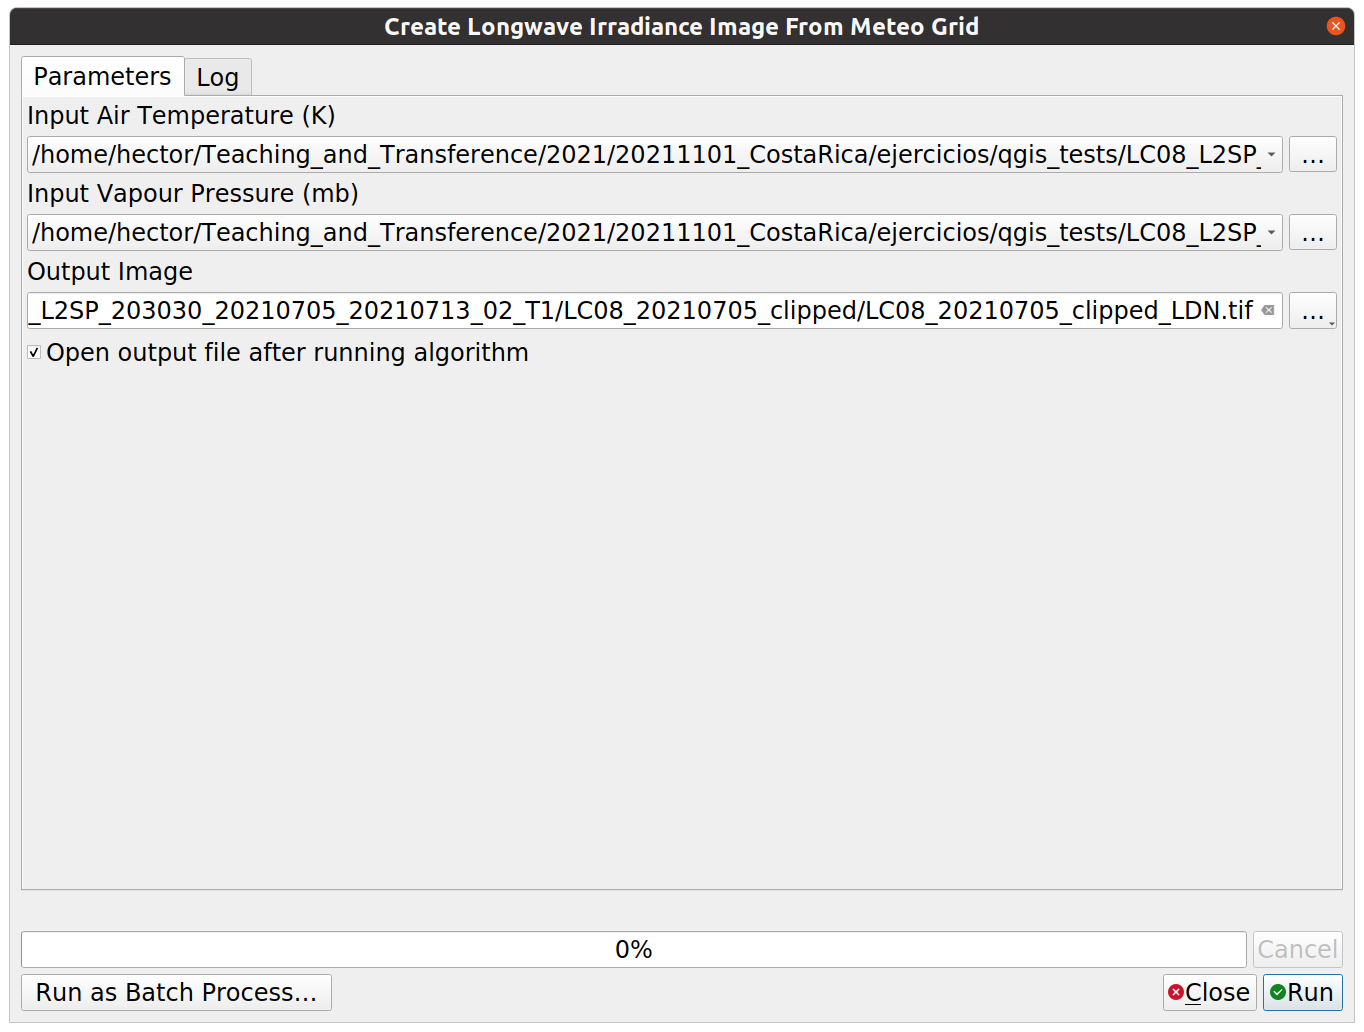
\includegraphics[width=\textwidth]{qgis_ldn_from_grid}
     \end{figure}
     
     \item Selecciona la imagen de temperatura del aire recortada (archivo con sufijo \cverb+TA+) en \cverb+Input Air Temperature (K)+
     
     \item Selecciona la imagen de presión de vapor del aire recortada (archivo con sufijo \cverb+EA+) en \cverb+Input Vapour Pressure (mb)+
     
     \item Selecciona un nombre para el archivo de salida en \cverb+Output Image+
    \end{enumerate}
    
    Con esto terminamos la parte principal de preparación de datos. Lo siguente ya apenas es ejecutar el modelo TSEB indicándole los inputs correspondientes e interpretar las salidas del modelo.
   
   \subsection{Ejecución del modelo TSEB}
    Con todos los datos ya preparados y alineados ya sólo tenemos que ejectuar nuestra función \cverb+TSEB+ y mirar las distintas variables que nos devuelve:
    
    \begin{enumerate}
     \item Ejecuta la función \cverb+TSEB: Two Source Energy Balance Model+, dentro del grupo \cverb+Evapotranspiration Models+ de nuestro complemento \cverb+Evapotranspiration Processor+.
     
     \begin{figure}[H]\centering
      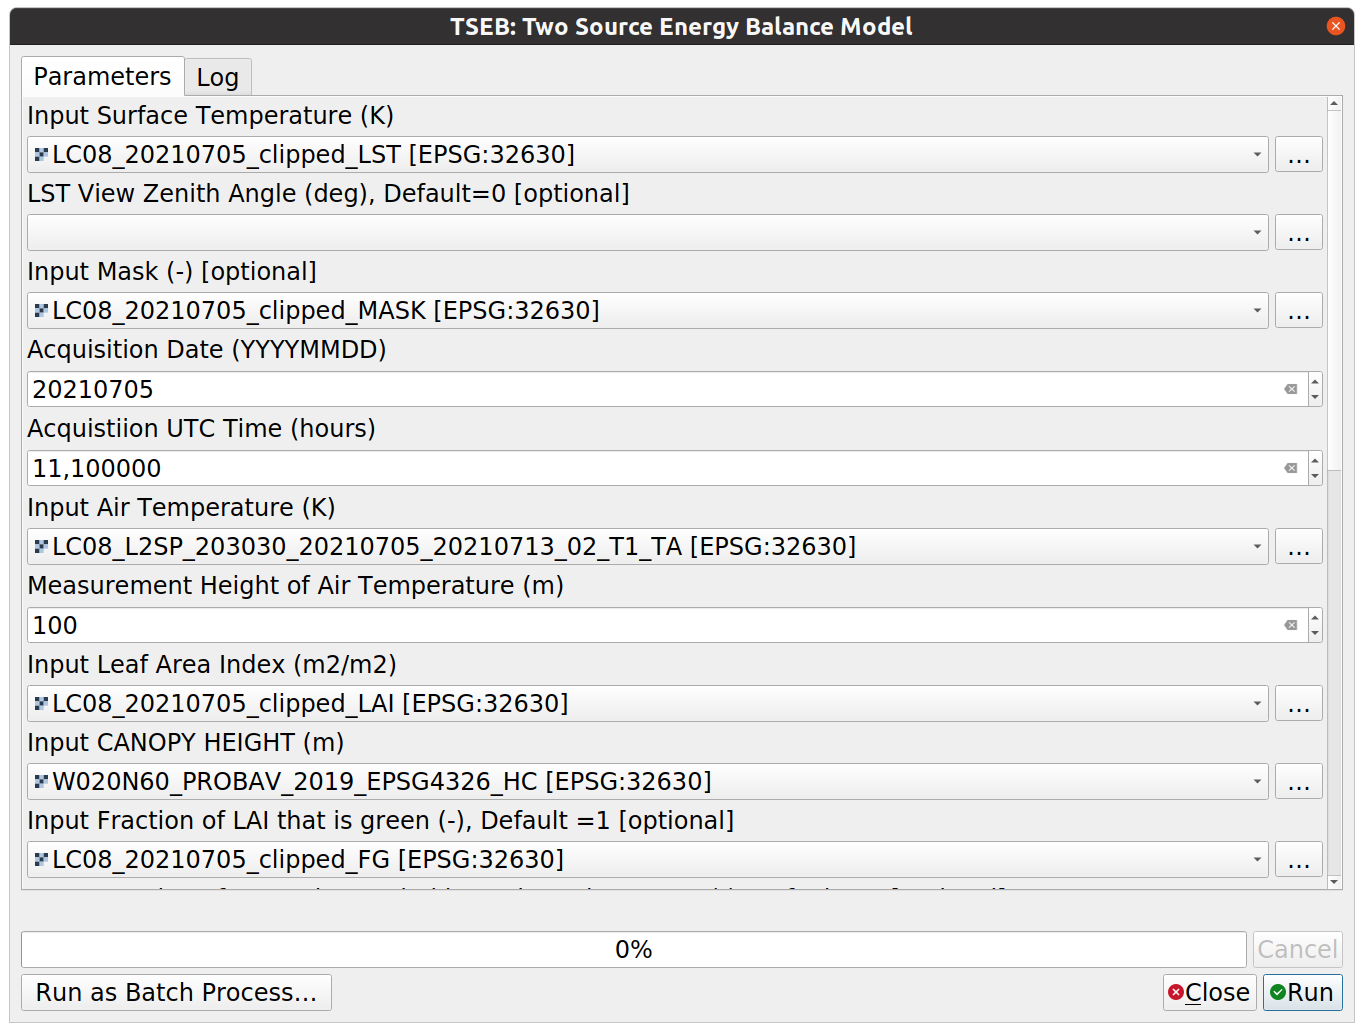
\includegraphics[width=\textwidth]{qgis_tseb_1}
      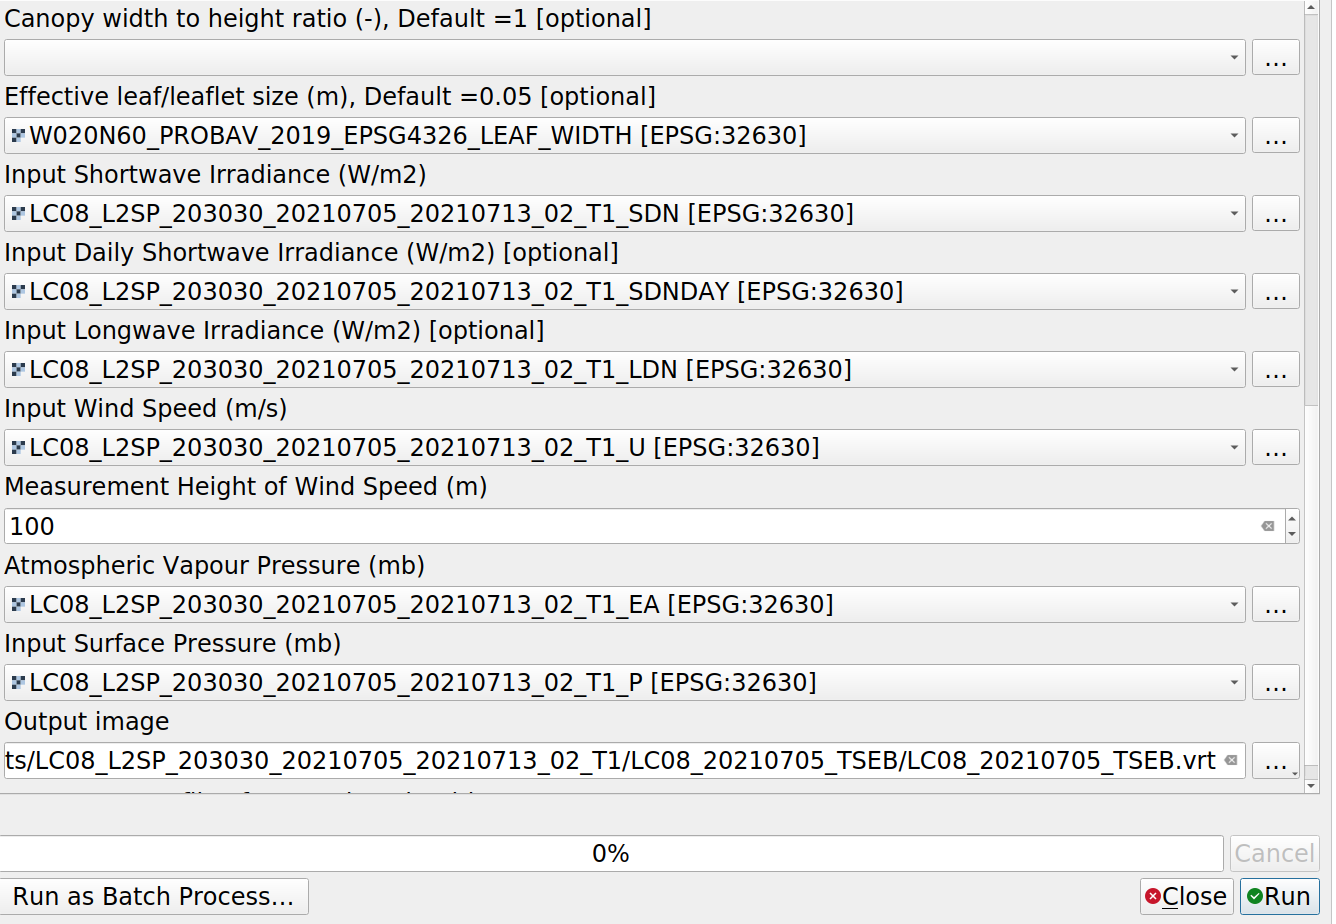
\includegraphics[width=\textwidth]{qgis_tseb_2}
     \end{figure}
     
     \item como verás hay un gran número de inputs a introducir, pero afortunadamente ya tenemos todos los inputs que necesitamos listos.
     \begin{itemize}
      \item La temperatura de superficie en \cverb+Input Surface Temperature (K)+.
      
      \item Deja en blanco \cverb+LST View Zenith Angle+ ya que asumimos que la observación de Landsat es prácticamente hacia el nadir (VZA=0).
      
      \item La máscara de nubes en \cverb+Input Mask+.
      
      \item La fecha de adquisición de la imagen en formato añomesdía en \cverb+Acquisition Date+.
      
      \item La hora de adqusición en UTC y en hora decimal (p.ej. 10.5 para las 10:30) en \cverb+Acquisition UTC Time+.
      
      \item La temperatura del aire (\cverb+TA+) en \cverb+Input Air Temperature (K)+.
      
      \item La altura de referencia de la temperatura del aire en \cverb+Measurement Height of Air Temperature (m)+. En el caso de nuestra práctica y si recuerdas el ejercicio de la práctica 5, la altura de referencia fue fijada en 100m sobre el nivel del terreno. Asegúrate que esta altura es siempre superior a la altura de tu dosel.
      
      \item El LAI en \cverb+Input Leaf Area Index+.
      
      \item La altura del dosel, generada a partir del mapa de tipos de cobertura, o cualquier otra fuente, en \cverb+Input Canopy Heght (m)+.
      
      \item En \cverb+Input Fraction of LAI that is green+ puedes dejarlo en blanco, asumiendo que durante el periodo vegetativo tu vegetación está completamente verde. Esta es una variable complidada de estimar y sólo es relevante durante la senescencia del cultivo. También puede estimarse de manera aproximada como el ratio $f_g=fAPAR/fIPAR$.
      
      \item Si tu zona incluye áreas con doseles significativamente heterogéneos como cultivos en hilera o árboles/plantas asiladas, introduce un mapa (p.ej. en base a un mapa de tipo de cobertura) con este valor. Si no puedes dejarlo en blanco y asumir que tu vegetación ocupa homogéneamente el terreno.
      
      \item Deja en blanco la opción \cverb+Canopy width to height ratio+. Esta opción sólo es efectiva si tu dosel no cubre todo el terreno. Se trata de un factor de forma del dosel, por defecto usa el valor ``1'' indicando que las copas individuales son de forma más o menos globosa. Si la anchura de la copa es significativamente distinta a la altura de la copa, entonces puedes plantearte generar esta información.
      
      \item Introduce tu mapa de tamaño efectivo de la hoja, que generamos gracias a nuestro mapa de tipos de cobertura, en \cverb+Effective leaf/leaflet size (m)+. En cualquier caso este parámetro no suele ser muy relevante a no ser que se trate de hojas muy grandes o muy finas y estrechas.
      
      \item La irradiancia solar a la hora de adqusición (\cverb+SDN+) va en \cverb+Input Shortwave Irradiance (W/m²)+.
      
      \item La irradiancia solar diara (\cverb+SDNDAY+) va en \cverb+Input Daily Shortwave Irradiance (W/m²)+. Esta variable es opcional, y se usa para extrapolar el flujo de calor sensible instantáneo ($\lambda E_i$ W/m²) a la ET diaria (mm/día).
      
      \item En \cverb+Input Longwave Irradiance+ introduce la irradiancia de onda larga. Esta variable es opcional, si no la introduces el modelo la calculará internamente.
      
      \item Introduce la velocidad del viento \cverb+U+ en \cverb+Input Wind Speed (m/s)+.
      
      \item Al igual que con la temperatura del aire, tenemos que introducir la altura de referencia de esta velocidad del viento. Al generar esta información a partir de nuestra función para descargar y procesar datos de Copernicus, la altura sería de 100 m.
      
      \item En \cverb+Atmospheric Vapour Pressure (mb)+ introduce la presión de vapor de agua (\cverb+EA+).
      ç
      \item En \cverb+Input Surface Pressure (mb)+ introduce la presión atmosférica (\cverb+P+).
      
      \item Finalmente introduce un archivo de salida donde guardar las estimaciones del modelo. En este caso es mejor guardar el archivo como formato \cverb+VRT+ en lugar de GeoTiff, ya que de esta manera cada salida del modelo será una imagen individual y será más facil ver cada producto generado.
     \end{itemize}
     
     \item Cuando hayas introducido todos los parámetros presiona en \cverb+Run+. Según el tamaño de tu imagen el algoritmo tardará más o menos.
    \end{enumerate}

    Al terminar de procesar, y si has guardado el archivo de salida como formato \cverb+VRT+, el algoritmo habrá generado una serie de imágenes en dos subcarpetas (\cverb+*.data+ \cverb+*_ancillary.data+). La información más relevante se encuentra en \cverb+*.data+, mientras que \cverb+*_ancillary.data+ muestra salidas del modelo auxiliares de menor utilidad.
    
    \begin{enumerate}
     \item \cverb+*.data+ contiene:
     
     \begin{figure}[H]\centering
      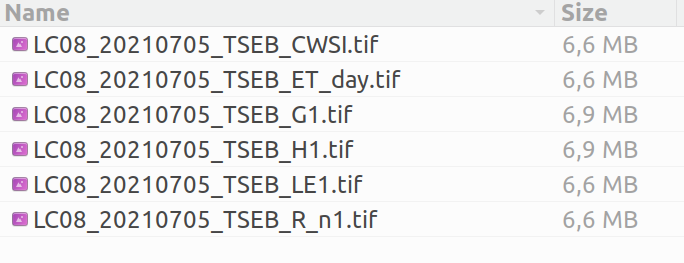
\includegraphics[width=\textwidth]{pytseb_data_folder}
     \end{figure}

     \begin{itemize}
      \item \cverb+LE1.tif+, el flujo de calor latente instantáneo, $\lambda E$ (W/m²).
      
      \item Si has incluido como variable de entrada la irradiancia solar diaria el algoritmo también incluye la ET diaria en la imagen \cverb+ET_day+ (mm/día).
      
      \item \cverb+CWSI.tif+, un índice de estrés hídrico (Crop Water Stress Index) calculado como el ratio entre el flujo de calor latente (o ET) actual ($\lambda E$) y potencial ($CWSI=1 - \frac{\lambda E}{\lambda E_0}$). CWSI típicamente muestra valores en torno a 0 si el cultivo está bien irrigado ($\lambda E \approx \lambda E_0$) y aumenta hacia 1 si éste se encuentra estresado ($\lambda E \approx 0$). 
      
      \item \cverb+H1.tif+, el flujo de calor sensible instantáneo (W/m²).
      
      \item \cverb+R_n1.tif+, la radiación neta instantánea (W/m²).
      
      \item \cverb+G1.tif+, el flujo de calor del suelo instantáneo (W/m²).
     \end{itemize}
     
     \item \cverb+*._ancillary_data+ contiene:
     
     \begin{figure}[H]\centering
      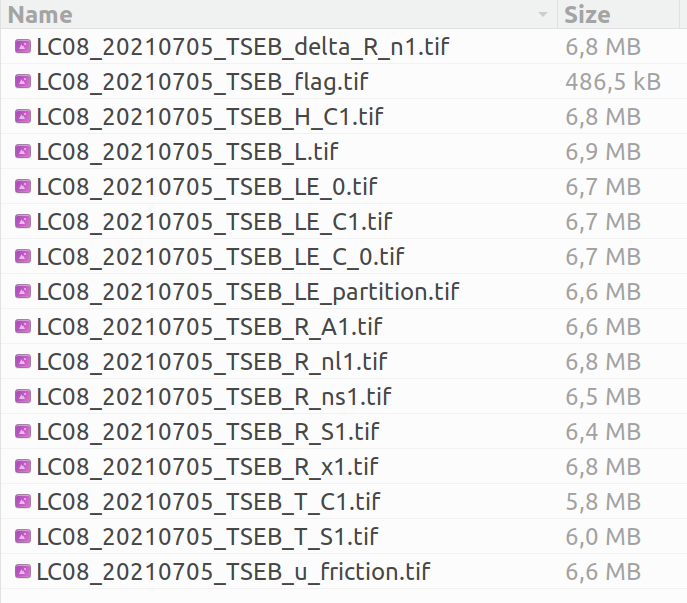
\includegraphics[width=\textwidth]{pytseb_ancdata_folder}
     \end{figure}
     
     de las que destacamos:
     \begin{itemize}
      \item \cverb+LE_partition.tif+, la fracción de transpiración con respecto a la ET (T/ET) estimado por TSEB.
      
      \item \cverb+LE_C.tif+, el flujo de calor latente de la vegetación (o la transpiración de la planta) estimado por TSEB (W/m²).
      
      \item \cverb+LE_O.tif+, el flujo de calor latente potencial estimado por Shuttleworth-Wallace (W/m²).
      
      \item \cverb+LE_C_O.tif+, el flujo de calor latente potencial de la planta estimado por Shuttleworth-Wallace (W/m²).
      
      \item \cverb+T_C1.tif+, la temperatura efectiva de las hojas estimada por TSEB (K).
      
      \item \cverb+T_S1.tif+, la temperatura del suelo estimada por TSEB (K).
      
      \item \cverb+R_ns1.tif+, la radiación neta de onda corta estimada por TSEB (W/m²).
      
      \item \cverb+R_ns1.tif+, la radiación neta de onda larga estimada por TSEB (W/m²).
     \end{itemize}
    \end{enumerate}
 
\section{Rellenado de huecos e interpolación temporal}
  Para finalizar con esta parte de Evapotranspiración, y pensando en aplicaciones de contabilidad de agua y cambios en la eficiencia del uso del agua a escalas temporales mayores (meses, años, ...). Puede ser de interés generar series temporales continuas de ET diaria. El reto consiste en que las imágenes de satélite van a contener huecos e incluso va a haber días sin acceso a ninguna imágen, en el caso de usar Landsat, por ejemplo.
  
  Aquí veremos un método sencillo a la hora de rellenar huecos e interpolar temporalmente las estimaciones de ET de teledetección. Se basa en el cálculo de un índice de estŕes del cultivo $K_{cs}$:
  
  \begin{equation*}
   K_{cs}^{(i)} = \frac{ET}{ET_{ref}^{(i)}}
  \end{equation*}
  donde $K_{cs}^{(i)}$ puede equipararse a la combinación del coeficiente de cultivo ($K_c$) y el coeficiente de estrés ($K_s$).
  
  De modo que la ET para un píxel sin datos en un día posterior (i+t) se podría calcular como:
  \begin{equation*}
   ET^{(i+t)} = K_{cs}^{(i)} ET_{ref}^{(i+t)} 
  \end{equation*}  
  mientras que para ese mismo día si otros píxeles si tienen dato válido de ET, su $K_{cs}$ puede actualizarse ($K_{cs}^{(i+t)} = ET^{(i+t)} / ET_{ref}^{(i+t)}$).
  
  La principal limitación de este método es que asume que entre imagen e imagen las condiciones del cultivo apenas han cambiado, por lo que tanto su fisiología como su grado de estrés hídrico son similares entre imágenes válidas. Esto  puede ser un hándicap importante en áreas con gran nubosidad y/o con observaciones poco frecuentes.
  
  El método requiere un mapa previo de $K_{cs}$, que se va actualizando, píxel a píxel, conforme se obtienen observaciones libres de nubes para cada píxel. Es por ello que este método require de cierto ``calentamiento'' y generar mapas de ET y $K_{cs}$ uno o varios meses antes del periodo de interés. En nuestro caso, como de momento sólo hemos trabajado con una fecha los resultados no son suficientemente robustos ya que necesitarías generar más mapas de ET con adquisiciones consecutivas (como por ejemplo descargar y procesar todas las imágenes Landsat dentro de un periodo de tiempo, contengan o no nubes). En cualquier caso, el método está implementado como otra función sencilla que podemos poner en práctica:
  
  \begin{enumerate}
   \item Ejecuta la función \cverb+Fill gaps in ET maps+ dentro del grupo \cverb+Evapotranspiration Models+.
   \begin{figure}[H]\centering
    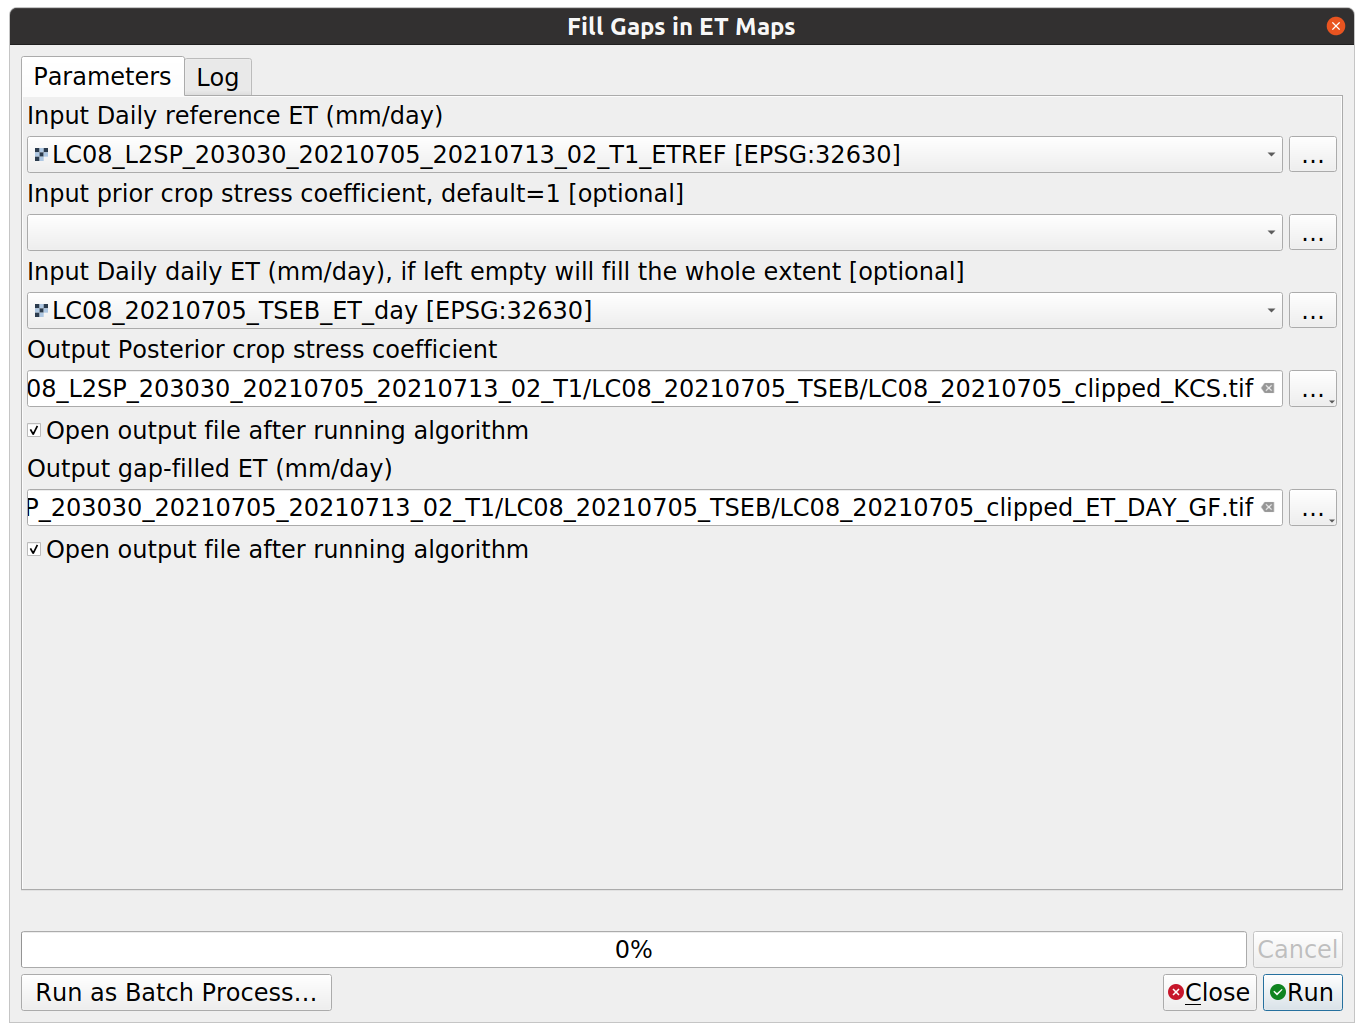
\includegraphics[width=\textwidth]{qgis_et_gap_fill}
   \end{figure}
   
   \item En \cverb+Input Daily Reference ET (mm/day)+ introduce el mapa de la ET de referencia diaria que generamos con los datos ECWMF y que ya está recortado y ajustado a nuestra área de interés.
   
   \item En \cverb+Input prior crop stress coefficient+ se introduciría el mapa de $K_{cs}$ de un día previo. Como en este caso no tenemos procesada más que una adquisición puedes dejarlo en blanco. El algoritmo asumirá entonces que para todos los píxeles sin dato $K_{cs}=1$. 
   
   \item En \cverb+Input prior crop stress coefficient+ se introduciría el mapa de $K_{cs}$ de un día previo. Como en este caso no tenemos procesada más que una adquisición puedes dejarlo en blanco. El algoritmo asumirá entonces que para todos los píxeles sin dato $K_{cs}=1$.
   
   \item En \cverb+Input Daily ET (mm/day)+ introduce nuestro mapa de ET diaria que acabamos de generar. 
   
   \item En \cverb+Output posterior crop stress coefficient+ indica un archivo de salida donde se guardará el mapa de $K_{cs}$ correspondiente a la fecha en la que estás trabajando.
   
   \item En \cverb+Output gap-filled ET (mm/day)+ indica un archivo de salida donde se guardará el mapa de ET diaria con todos los huecos rellenados.
  \end{enumerate}

  Verás que si tu imagen tenía alguna nube (y por tanto \cverb+ET_day+ no tenía dato), con el nuevo mapa guardado en \cverb+Output gap-filled ET (mm/day)+ esos huecos ya estarán rellenos. Además, tendrás un mapa de $K_{cs}$ que podrás utilizar para rellenar huecos de días posteriores.
  
  Cuantas más fechas e imágenes generes, sobre todo si en tu zona no hay excesivas nubes recurrentemente, la calidad del rellenado de los huecos será mejor. Con este método puedes generar mapas diarios de ET, para luego agregarlos para un periodo de tiempo (semanal, mensual, anual, ...) y así tener una estimación del consumo de agua por parte del cultivo para esos periodos de tiempo.
    
\end{document}
